% CODIGO DE ORDENACIONES
\definecolor{lightergray}{RGB}{247,247,247}
\definecolor{darkgreen}{RGB}{36,135,20}
\definecolor{green_comment}{RGB}{0,128,0}
\definecolor{redcell}{RGB}{238,176,176}
\definecolor{greencell}{RGB}{217,234,211}
\definecolor{lightblack}{RGB}{159,159,152}



\chapter{Estudio empírico}
\label{cap:c4_estudio}	
Después de diseñar e implementar las estrategias descritas en la Sección \ref{cap:c3_implementaciones}, llevamos a cabo un análisis exhaustivo para evaluar los tiempos de ejecución de cada una, así como contrastar resultados y extraer conclusiones

Primero, se ejecutan los experimentos en un ordenador de propósito general. Seguidamente se ejecutan las mejores implementaciones en un sistema distribuido con un número elevado de núcleos de CPU. 

\section{Entornos de ejecución}

Para ejecutar los experimentos y comprobar el funcionamiento de las implementaciones, primero se ejecutan en un ordenador de propósito general. Este sistema computacional tiene las siguientes especificaciones:

\begin{itemize}
	\item Procesador (CPU): \textit{AMD Ryzen 7}, con 8 núcleos y 16 hilos, a 4.20 GHzs
	\item Memoria (RAM): 32 GB de \textit{RAM DDR4}, permitiendo una amplia capacidad para manejar grandes volúmenes de datos en memoria. Característica fundamental para ejecutar algoritmos de IA que demandan una cantidad elevada de recursos.
	\item Tarjeta Gráfica (GPU): \textit{NVIDIA GeForce RTX 3070} con arquitectura \textit{Ampere} \cite{pool2020accelerating}, que cuenta con 5888 núcleos CUDA y 8 GB de memoria GDDR6. La arquitectura \textit{Ampere} es sucesora de la arquitectura \textit{Turing} lanzada en 2020. Fue diseñada para brindar un mejor rendimiento, especialmente en aplicaciones de computación paralela.
	\item Placa Base: \textit{X570 Gaming}. Soporta las tecnologías de conectividad de alta velocidad, garantizando el rendimiento y estabilidad del sistema en condiciones de carga elevada.
\end{itemize}

El sistema distribuido consta de tres ordenadores. Uno que funciona de Front-End y dos como nodos de cómputo, sumando entre estos últimos 128 núcleos de CPU y 256 GB de RAM. La figura \ref{fig:cluster} muestra la estructura del \textit{cluster}.




El Front-End realiza la conexión remota con los otros dos ordenadores, situados en la Facultad de Informática de la Universidad Complutense de Madrid. Este ordenador no participa en el cómputo, solo mantiene los \textit{scripts} (tipo de fichero de texto con el código escrito en un lenguaje de programación, en este caso Python) y lanza los experimentos sobre los nodos de cómputo.  Durante las pruebas, cada proceso tiene un núcleo dedicado, por lo que el rendimiento de cada proceso no se ve afectado por otros procesos del sistema. Esto permite mayor precisión para evaluar el rendimiento del sistema, y las pruebas ejecutadas no compiten por los recursos de la CPU. 


\vspace*{0.2cm}

\begin{figure}[!h]
	\centering
	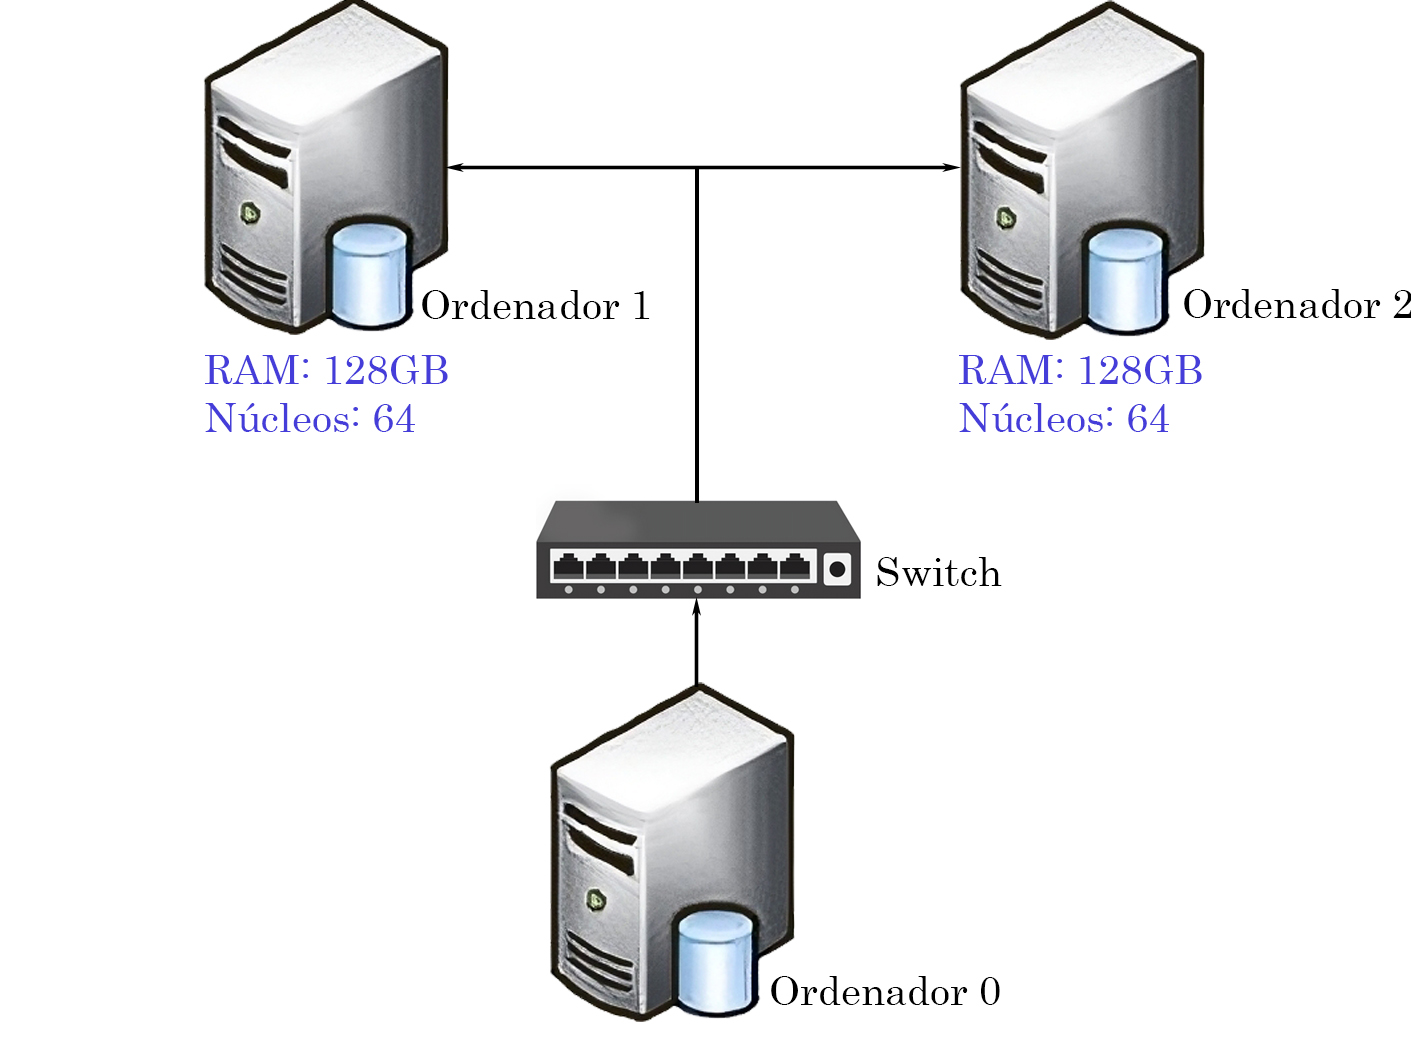
\includegraphics[width=0.5\textwidth]{images/chapter_4/cluster}
	\caption{Estructura del sistema distribuido de la Facultad de Informática}
	\label{fig:cluster}
\end{figure}


Para realizar las pruebas se usan las funciones \textit{open()} y \textit{write()} de Python para almacenar los tiempos de ejecución en ficheros de texto. Los tiempos se miden con las funciones de
tiempo de MPI, MPI.Wtime().

\section{Programas sencillos}

Primero realizamos el estudio de los programas básicos descritos en la Sección \ref{cap:c3_1}, ordenación de arrays y multiplicación de matrices.

% ------------------------------------------------------------------------------------------------
% --- ORDENACIONES  ------------------------------------------------------------------------------
% ------------------------------------------------------------------------------------------------
\subsection{Ordenaciones}

Las pruebas realizadas para estos algoritmos se realizan para el peor de los casos, es decir, un array de enteros sin repeticiones ordenado de forma decreciente. Cada algoritmo tiene que realizar el mayor número de comparaciones posible para ordenar el array de manera creciente. El resultado de cada experimento (tiempo de ejecución en segundos) es almacenado en un fichero de texto. Seguidamente se aumenta el tamaño del array para ejecutar el siguiente experimento, hasta llegar a \textit{100.000} elementos.	

\subsubsection{Algoritmos de complejidad cuadrática}		
\label{cap:4_2_1_1}

Debido al coste cuadrático de estos algoritmos, el incremento entre pruebas del tamaño de los arrays se obtiene de la siguiente forma:
\begin{itemize}
	\vspace*{-0.2cm}	
	\item \([20-1.000)\) $\rightarrow$ 20 elementos.
	\vspace*{-0.4cm}	
	\item \([1.000-10.000)\) $\rightarrow$ 250 elementos.
	\vspace*{-0.4cm}	
	\item \([10.000-100.000)\) $\rightarrow$ 1.000 elementos.					
\end{itemize}


%\subsubsection{Algoritmo \textit{SequentialSort} aplicando las estrategias de HPC}			

\textit{SelectionSort} es fácilmente paralelizable, pues para cada elemento se comprueba cuantos elementos en el array son mayores. Las estrategias implementadas utilizan el modelo \textit{Master-Worker}. El \textit{master} envía a cada proceso \textit{worker} un elemento del array para que hagan las comparaciones y devuelvan el índice del elemento, junto con el número de elementos mayores que el recibido, y así el \textit{master} se encarga de ordenar el array y enviar elementos sin procesar. La Figura \ref{fig:sequentialsort_mpi} muestra los tiempos de ejecución. En rojo el algoritmo sin mejora, y en verde y negro las dos estrategias ejecutadas con cinco procesos. Se puede apreciar una considerable reducción del tiempo de ejecución. 

Al comparar las dos estrategias MPI, se obtiene que la primera estrategia es un \textit{34\%} más rápida que la segunda. Sin embargo, la segunda estrategia tiene una menor complejidad espacial, mostrando en la gráfica de la derecha, en negro, que la memoria no varía al aumentar los procesos ejecutados.

% Sequential sort + Uso de memoria
\begin{figure}[h!]
	\centering
	\begin{tikzpicture}
		\begin{groupplot}[group style={
				group size=2 by 1,
				horizontal sep=1.5cm, 
				vertical sep=0.5cm}, 
			grid=major,
			width=0.5\textwidth, height=0.37\textwidth, 
			tick label style={font=\tiny}
			]
			
			% Grafico de la izquierda --------------
			\nextgroupplot[
			title={}, 
			ylabel=Tiempo de ejecución (s), 
			xlabel=Tam. Array ($10^4$),
			legend pos=north west,					
			scaled x ticks=false,
			]
			\addplot [mark=none, color=red, line width=1.2pt] table [x index=0, y index=1, col sep=space] {files/sequential.txt};
			\addplot [mark=none, color=darkgreen, line width=1.2pt] table [x index=0, y index=2, col sep=space] {files/sequential.txt};
			\addplot [mark=none, color=black, line width=1.2pt] table [x index=0, y index=3, col sep=space] {files/sequential.txt};
			
			% Leyendas
			\addlegendentry{Secuencial}
			\addlegendentry{MPI\_1}
			\addlegendentry{MPI\_2}
			
			% Grafico de la derecha --------------
			\nextgroupplot[
			title={},
			xtick={2,3,4,5,6,7,8,9,10}, 
			ytick={0,2,4,6,8,10,12}, 
			legend pos=north west,			
			xlabel=Num. Procesadores,
			ylabel=Memoria \tiny(Copias del array)
			]
			\addplot[name path=darkgreen, color=darkgreen, mark=square] table {files/sequentialMem.txt};
			
			
			\addplot[name path=black, color=black, mark=triangle] table [y index=2] {files/sequentialMem.txt};
			
			
			\addplot [color=darkgreen!50, fill=darkgreen!50, fill opacity=0.3] fill between [of=darkgreen and black, soft clip={domain=2:10}];
			
			\addplot [name path=axis, draw=none] coordinates {(2,0) (10,0) };	
			
			\addplot [color=black!50, fill=black!50, fill opacity=0.3] fill between [of=black and axis, soft clip={domain=2:10}];
			
			% Leyendas
			\addlegendentry{MPI\_1}
			\addlegendentry{MPI\_2}
			
		\end{groupplot}  				
	\end{tikzpicture}
	\caption{Tiempos de ejecución de las estrategias y su uso de Memoria para el algoritmo \textit{SequentialSort} en ordenador de propósito general}
	\label{fig:sequentialsort_mpi}
\end{figure}



%Primero ejecutamos las pruebas para los algoritmos sin mejora, comprobando así cual es el mejor.

Una vez comparadas las estrategias con el algoritmo secuencial, podemos comprobar el rendimiento frente a los algoritmos conocidos. La Figura \ref{fig:ordenaciones_cuadraticas} muestra que \textit{SelectionSort} (la línea negra) es la ordenación que mejores resultados obtiene, y \textit{BubbleSort} (línea roja) la que peores. \textit{SelectionSort} es, aproximadamente, \textit{3.5} veces más rápida al ordenar \textit{70.000} elementos. La ordenación \textit{SequentialSort} sin paralelizar, es incluso más rápida que dos de las más conocidas. Esto es debido a la simpleza de las operaciones aplicadas en la ordenación, pues solo hace \(N^{2}\) comparaciones. En \textit{BubbleSort} e \textit{InsertionSort}, además de realizar comparaciones, modifican las posiciones de los elementos en el array, aumentando el tiempo de ejecución.

La estrategia MPI de \textit{SequentialSort} que menos tiempo requiere (la primera) no obtiene mejores resultados que la mejor ordenación sin mejoras (\textit{SelectionSort}) hasta llegar a los cuatro procesadores, siendo un \textit{20\%} más veloz. Para mostrar de forma más clara la diferencia de tiempos entre estas dos ordenaciones, se muestra la ejecución de la primera estrategia con cinco procesadores (Sequential\_MPI(5)), obteniendo un \textit{50\%} de mejora.


\begin{figure}[!h]
	\centering
	\begin{tikzpicture}
		\begin{axis}[
			xlabel={Tam. Array ($10^4$)},
			ylabel={Tiempo de ejecución (s)},
			xtick={0,1,2,3,4,5,6,7,8},
			legend pos=north west,
			grid=major,
			width=0.70\textwidth,
			height=0.4\textwidth,
			scaled x ticks=false,
			]				
			
			\addplot [mark=none, color=red, line width=1.2pt] table [x index=0, y index=1, col sep=space] {files/sortn2.txt};
			\addplot [mark=none, color=blue, line width=1.2pt] table [x index=0, y index=2, col sep=space] {files/sortn2.txt};
			\addplot [mark=none, color=black, line width=1.2pt] table [x index=0, y index=3, col sep=space] {files/sortn2.txt};
			\addplot [mark=none, color=magenta, line width=1.2pt] table [x index=0, y index=4, col sep=space] {files/sortn2.txt};
			\addplot [mark=none, color=darkgreen, line width=1.2pt] table [x index=0, y index=5, col sep=space] {files/sortn2.txt};
			
			
			\addlegendentry{Bubble}
			\addlegendentry{Insertion}
			\addlegendentry{Selection}
			\addlegendentry{Sequential}
			\addlegendentry{Sequential\_MPI(5)}
			
		\end{axis}
	\end{tikzpicture}
	\caption{Tiempo de ejecución de los algoritmos de ordenación cuadráticos en ordenador de propósito general}
	\label{fig:ordenaciones_cuadraticas}
\end{figure}


\subsubsection{Algoritmo \textit{MergeSort}}

Este algoritmo no tiene un coste tan elevado como los anteriores. La complejidad es logarítmica O(NLogN) lo que provoca que se pueda aumentar el tamaño del array a ordenar. Para la estrategia implementada, no se aplica el modelo \textit{Master-Worker}, sino que todos los procesos creados trabajan de manera equitativa. Como se dijo en la Sección \ref{cap:c3_1}, esta estrategia usa potencias de dos procesos para ordenar el array. En cada iteración los procesos se comunican con el más cercano, uno le envía su subarray ordenado y termina su ejecución (el de mayor \textit{id} de cada pareja), mientras que el otro reordena los dos subarrays y continúa a la siguiente iteración.


En esta ocasión, la prueba realizada consiste en ordenar de manera creciente cuatro arrays de enteros inicializados de manera decreciente (peor de los casos), empezando con \textit{25.000} elementos e incrementando esa misma cantidad entre los experimentos. Pese a tener solo ocho núcleos en el ordenador de propósito general, se comprueba el rendimiento de la estrategia con \textit{4}, \textit{8}, \textit{16} y \textit{32} procesos. La Figura \ref{fig:mergesort_hist} muestra los resultados obtenidos en forma de histograma. Como la estrategia aplica ordenaciones cuadráticas en los subarrays al comienzo del algoritmo, no se obtienen buenos resultados con pocos procesos, debido al elevado tamaño del array a ordenar. Con dos procesos no reduce el tiempo de ejecución, lo duplica. El cómputo es equivalente a aplicar una ordenación cuadrática con la mitad del array a ordenar. No obstante, se puede apreciar una notoria reducción del tiempo de ejecución a partir de \textit{16} procesos, llegando a tener un \textit{speed-up} aproximado de \textit{15.5}. Es cierto que se podrían aplicar otras ordenaciones con menor complejidad para reducir más el tiempo, pero así se demuestra que en la computación de alto rendimiento se pueden obtener buenos resultados con estrategias no tan efectivas, pero bien paralelizadas.

% HISTOGRAMA CON VARIOS PROCESOS
\begin{figure}[!h]
	\begin{tikzpicture}
		\begin{axis}[
			ybar,
			bar width=0.35cm,
			ylabel={Tiempo de ejecución (s)},
			xlabel={Tam. array ($10^3$)},
			symbolic x coords={25, 50, 75, 100},
			xtick=data,
			enlarge x limits=0.2,
			ymin=0,
			%width=15cm,
			%height=10cm,
			width=\textwidth,
			height=0.38\textwidth,
			legend style={at={(0.5,1.16)}, anchor=north, legend columns=-1},
			area legend
			]
			
			\addplot+[ybar, pattern=vertical lines, draw=black] plot coordinates 
			{(25, 1.12) (50, 4.39) (75, 10.0) (100, 21)};
			\addplot+[ybar, pattern=grid, draw=black] plot coordinates 
			{(25, 0.67) (50, 2.58) (75, 5.70) (100, 10.15) };
			\addplot+[ybar, pattern=dots, draw=black] plot coordinates 
			{(25, 0.23) (50, 0.93) (75, 2.09) (100, 3.35) };
			\addplot+[ybar, pattern=crosshatch, draw=black] plot coordinates 
			{(25, 0.09) (50, 0.34) (75, 0.72) (100, 1.39)};
			\addplot+[ybar, pattern=checkerboard, draw=black] plot coordinates 
			{(25, 0.059) (50, 0.18) (75, 0.41) (100, 0.71)};
			
			
			\legend{Secuencial, MPI(4),MPI(8),MPI(16),MPI(32)}
		\end{axis}	
	\end{tikzpicture}
	\caption{Tiempo de ejecución del algoritmo \textit{MergeSort} en ordenador de propósito general}
	\label{fig:mergesort_hist}
\end{figure}



La memoria está optimizada, puesto que el array está dividido entre los procesos. Al terminar un proceso con la sincronización en mariposa comentada en la Sección \ref{cap:c3_1}, se termina la ejecución del proceso liberando memoria una vez ha enviado al proceso correspondiente su subarray ordenado.



%%\subsubsection{Cluster}
Seguidamente, pasamos a comentar las pruebas realizadas en el sistema distribuido.

El algoritmo secuencial de \textit{MergeSort} tarda unos \textit{20.16} segundos en ordenar, de manera creciente, un array de \textit{100.000} elementos ordenados de manera decreciente (el peor de los casos). Por ello, realizamos un experimento para saber cuánto tiempo requiere la estrategia en ordenar un array con un millón de elementos. Las pruebas comienzan con \textit{100.000} elementos, incrementando nueve veces su tamaño hasta llegar al millón de elementos. Estas pruebas se realizan con \textit{16}, \textit{32}, \textit{64} y \textit{128} procesos. La Figura \ref{fig:mergesort_cluster} muestra los resultados obtenidos. 

De manera secuencial, sin mejoras, el algoritmo requiere \textit{20.16} segundos en ordenar \textit{100.000} elementos, mientras que con 128 procesos requiere \textit{0.16} segundos, obteniendo un \textit{speed-up} de \textit{125}. 

\begin{figure}[!h]
	\hspace{-0.07\textwidth}
	\begin{tikzpicture}
		\begin{axis}[
			xlabel={Tam. Array ($10^5$)},
			ylabel={Tiempo de ejecución (s)},
			legend style={at={(1.02,0.5)}, anchor=west},
			grid=major,
			width=\textwidth,
			height=0.45\textwidth,				
			scaled x ticks=false,
			legend cell align={left},
			extra description/.code={
				\node at (1.01, 0.72) [anchor=west] {\textbf{Cores}};
			}
			]
			
			\addplot [mark=*, color=red, line width=1.2pt] table [x index=0, y index=1, col sep=space] {files/cluster/sort.txt};
			\addplot [mark=square*, color=blue, line width=1.2pt] table [x index=0, y index=2, col sep=space] {files/cluster/sort.txt};
			\addplot [mark=triangle*, color=black, line width=1.2pt] table [x index=0, y index=3, col sep=space] {files/cluster/sort.txt};
			\addplot [mark=star, color=darkgreen, line width=1.2pt] table [x index=0, y index=4, col sep=space] {files/cluster/sort.txt};
			
			
			\addlegendentry{16}
			\addlegendentry{32}
			\addlegendentry{64}
			\addlegendentry{128}
			
			
		\end{axis}
	\end{tikzpicture}
	\caption{Tiempo de ejecución del algoritmo \textit{MergeSort} en el Cluster}
	\label{fig:mergesort_cluster}
\end{figure}





% ------------------------------------------------------------------------------------------------
% --- MATRIZ -------------------------------------------------------------------------------------
% ------------------------------------------------------------------------------------------------
\subsection{Multiplicación de matrices}

Para este algoritmo, al contrario que los anteriores, no hay caso peor, pues siempre se ejecutan el mismo número de multiplicaciones para cualquier combinación de una matriz. 

Las pruebas se realizan con una única matriz cuadrada de tamaño \textit{1750}. Se genera de manera aleatoria con valores enteros que oscilan entre \textit{[1-9]}, y es almacenada para usar en cada prueba. Inicialmente, la matriz empieza con diez filas y columnas, al finalizar una prueba, se almacena el tiempo de ejecución y se incrementa el tamaño en diez, así hasta llegar a \textit{1750} filas y columnas. 

La distribución de tareas de los procesos se realiza mediante el modelo \textit{Master-Worker}. El proceso \textit{master} se encarga de enviar una matriz completa \textit{(B)} y filas de la matriz \textit{(A)} a los \textit{workers} para que realicen el cálculo. Al finalizar el procesado envían de vuelta el resultado al \textit{master} y esperan otras filas sin procesar, para poder, al final de la ejecución, formar entre todos la matriz final \textit{(C)}. \textit{(A*B=C)}

Cada proceso necesita, al menos, una copia de una matriz completa. El uso de memoria es proporcional al número de procesos ejecutados. No hace falta tener las dos matrices porque el \textit{master} se encarga de repartir filas para que vayan realizando el cálculo.

\vspace*{0.2cm}

Seguidamente, se ejecutan los programas de multiplicación de matrices en el ordenador de propósito general. La Figura \ref{fig:mult_matrices} muestra la ejecución del algoritmo secuencial, además de la estrategia implementada en la Sección \ref{cap:c3_1}, con \textit{2}, \textit{4} y \textit{6} procesos \textit{workers}. Se puede apreciar la reducción de tiempo, aplicando la estrategia con los diferentes números de procesos, llegando a obtener un \textit{speed-up} de \textit{8.4} al ejecutar el algoritmo con seis \textit{workers} en una multiplicación de \textit{1750x1750}.

\begin{figure}[!h]
	\centering
	\begin{tikzpicture}
		\begin{axis}[
			xlabel={Matriz (NxN)},
			ylabel={Tiempo de ejeución (s)},
			legend pos=north west,
			grid=major,
			width=\textwidth,
			height=0.4\textwidth
			]				
			
			\addplot [mark=none, color=red, line width=1.2pt] table [x index=0, y index=1, col sep=space] {files/multiplicacion1.txt};
			\addplot [mark=none, color=blue, line width=1.2pt] table [x index=0, y index=2, col sep=space] {files/multiplicacion1.txt};
			\addplot [mark=none, color=black, line width=1.2pt] table [x index=0, y index=3, col sep=space] {files/multiplicacion1.txt};
			\addplot [mark=none, color=darkgreen, line width=1.2pt] table [x index=0, y index=4, col sep=space] {files/multiplicacion1.txt};
			
			
			\addlegendentry{Secuencial}
			\addlegendentry{MPI(2)}
			\addlegendentry{MPI(4)}
			\addlegendentry{MPI(6)}
			
			
		\end{axis}
	\end{tikzpicture} 
	\caption{Tiempo de ejecución de multiplicación de matrices en ordenador de propósito general}
	\label{fig:mult_matrices}
\end{figure}



\newpage

Las oscilaciones en la gráfica se deben al incremento de diez elementos entre pruebas en un algoritmo con complejidad cúbica O($N^{3}$). Estas oscilaciones son más pronunciadas en la multiplicación sin paralelizar, pues el tiempo de ejecución es mayor.

En el \textit{cluster}, al poder ejecutar un número elevado de procesos, se puede aumentar el tamaño de las matrices de las pruebas a ejecutar. Utilizamos \textit{16}, \textit{32}, \textit{64} y \textit{128} procesos para medir el tiempo que tarda el algoritmo con la misma estrategia que la prueba anterior. En este caso, comenzando con \textit{500} elementos por fila, e incrementando ese mismo tamaño hasta llegar a una matriz de \textit{5000} filas y columnas. 

La Figura \ref{fig:mult_matrices_cluster} muestra los tiempos de ejecución con los procesos y tamaños comentados en el párrafo anterior. No se puede apreciar, pero con una matriz de \textit{1000} filas, ejecutar \textit{128} procesos reduce el tiempo de ejecución hasta unos \textit{1.06} segundos, logrando un \textit{speed-up} de \textit{84} con respecto a los \textit{89.1} segundos del cálculo sin paralelizar. La comunicación entre procesos no es tan optimizada como en la estrategia de \textit{MergeSort}, debido a que en esta implementación aplicamos el modelo \textit{Master-Worker} y es posible que un proceso \textit{worker}, al finalizar de procesar una fila, tenga que esperar a que el \textit{master} esté libre (puede estar recibiendo y colocando otros datos recibidos de otro proceso) para recibir nuevos datos que procesar. En cada experimento, se pierden \textit{(N/M)*T} segundos en la comunicación entre procesos. Siendo \textit{N} el número de filas de la matriz, \textit{M} el número de \textit{workers} y \textit{T} el tiempo de comunicación.

\begin{figure}[!h]
	%\centering % AL QUITAR ESTA OPCION SE PUEDE MOVER LA FIGURA
	\hspace{-0.07\textwidth} 
	\begin{tikzpicture}
		\begin{axis}[
			xlabel={Matriz (NxN)},
			ylabel={Tiempo de ejecución (s)},
			legend style={at={(1.02,0.5)}, anchor=west},
			grid=major,
			width=\textwidth, 
			height=0.45\textwidth,
			legend cell align={left},
			extra description/.code={
				\node at (1.01, 0.72) [anchor=west] {\textbf{Cores}};
			}
			]
			
			\addplot [mark=*, color=red, line width=1.2pt] table [x index=0, y index=1, col sep=space] {files/cluster/mult.txt};
			\addplot [mark=square*, color=blue, line width=1.2pt] table [x index=0, y index=2, col sep=space] {files/cluster/mult.txt};
			\addplot [mark=triangle*, color=black, line width=1.2pt] table [x index=0, y index=3, col sep=space] {files/cluster/mult.txt};
			\addplot [mark=star, color=darkgreen, line width=1.2pt] table [x index=0, y index=4, col sep=space] {files/cluster/mult.txt};
			
			\addlegendentry{16}
			\addlegendentry{32}
			\addlegendentry{64}
			\addlegendentry{128}
			
		\end{axis}
	\end{tikzpicture}
	\caption{Tiempo de ejecución de multiplicación de matrices en el Cluster}
	\label{fig:mult_matrices_cluster}
\end{figure}





% ------------------------------------------------------------------------------------------------
% --- JERARQUICO AGLOMERATIVO --------------------------------------------------------------------
% ------------------------------------------------------------------------------------------------


\section{Algoritmos de Agrupación}

Las poblaciones que se utilizan en las pruebas de esta sección se han almacenado en un fichero para usar la misma población generada de manera aleatoria, con dos variables de entrada, es decir, individuos es un plano bidimensional. Los valores son delimitados en el siguiente intervalo \textit{[-10, 10]}, ya que los valores no influyen en el cálculo de la distancia. Los tamaños de las poblaciones se incrementan dependiendo de la complejidad temporal de cada algoritmo. En sus secciones se especifica en profundidad.	

Los tres algoritmos de esta sección se basan en el modelo \textit{Master-Worker}. El \textit{master} divide los datos de entrada para que los \textit{workers} hagan el procesado. El \textit{master} en cada algoritmo tiene las siguientes funciones:	

\begin{itemize}
	\item Jerárquico Aglomerativo. En cada iteración se encarga de gestionar qué procesos tienen que eliminar o actualizar las filas y columnas de la matriz. El \textit{master} no tiene una copia de la matriz, mejorando así el uso de memoria al estar dividida entre los procesos \textit{workers}.
	\item KMedias. Su función principal es comprobar la condición de finalización. En cada iteración recibe las asignaciones de los datos procesados de los \textit{workers}, y si esta asignación no varía, se finaliza la ejecución.
	\item K-Vecinos más Cercanos (KNN). En las dos estrategias se encarga, de diferente forma, de actualizar las poblaciones de los \textit{workers} para que haya más precisión a la hora de categorizar nuevos individuos.
\end{itemize} 

%Los algoritmos de aprendizaje no supervisado, Jerárquico Aglomerativo y K-Medias, categorizan una población entera, y además tienen una complejidad cuadrática O(\(N^{2}\)). Por eso, para las pruebas, se incrementan las poblaciones de la siguiente forma:

%\begin{itemize}
%	\vspace*{-0.2cm}	
%	\item \([20-1.000)\) $\rightarrow$ 20 elementos.
%	\vspace*{-0.4cm}	
%	\item \([1.000-10.000)\) $\rightarrow$ 250 elementos.
%	\vspace*{-0.4cm}	
%	\item \([10.000-100.000)\) $\rightarrow$ 1.000 elementos.					
%\end{itemize}


\subsection{Jerárquico Aglomerativo}

De los tres algoritmos de agrupación, este es el más lento. Su bucle principal itera \textit{N-C} veces, siendo \textit{N} el número de individuos de la población y \textit{C} el número de \textit{clusters} deseados. En cada iteración, recorre una matriz entera para juntar dos \textit{clusters}, los que se encuentren a menor distancia. 

%\subsubsection{Distancias sin mejoras}		

En este algoritmo, el cálculo de las distancias entre \textit{clusters} es muy importante. Cada tipo genera diferentes agrupaciones, además de tener diferentes complejidades temporales. La distancia por \textit{centroides} es la que menos tiempo consume, siendo constante, al solo importar los centros de los clusters. Mientras que \textit{enlace simple} y \textit{completo} tienen una complejidad cuadrática O(\(N^{2}\)), recorriendo todos los individuos de ambos \textit{clusters} para calcular la distancia. Además, hay que añadir el cálculo de la distancia entre individuos, que puede ser \textit{Manhattan} o \textit{Euclídea}, siendo esta última un poco más costosa computacionalmente que la primera.


Para mostrar la importancia de las distancias entre \textit{clusters} y entre individuos, se realiza un estudio de los algoritmos sin aplicar ninguna estrategia computo de alto rendimiento (HPC). Con la población almacenada, se ejecutan las diferentes combinaciones de distancias (entre \textit{cluster} e individuo), generando 4 tipos, pues entre enlace \textit{simple} y \textit{completo} solo varía almacenar la menor o mayor distancia entre clusters. Empezando con veinte individuos, y aumentando ese mismo tamaño hasta llegar a mil. A partir de este punto, es mejor incrementar en \textit{250} individuos. La Figura \ref{fig:prueba_jerarquicosec} muestra los resultados de este experimento 

Al principio no hay tanta diferencia, pero conforme aumenta el tamaño de la población, los tiempos de ejecución empiezan a distinguirse. Como muestra el círculo rojo, la distancia entre \textit{clusters} por \textit{centroide} no varía mucho usar una distancia \textit{Euclídea} o \textit{Manhattan} entre individuos. No obstante, aplicando enlace \textit{simple} (o \textit{completo}) es mejor usar distancia \textit{Manhattan}. El cálculo de distancias entre individuos no usa potencias o raíces cuadradas, operaciones con un mayor coste que restas en valor absoluto. Cabe recalcar la diferencia de las distancias entre \textit{clusters} por \textit{centroide} y por enlace \textit{simple} y \textit{completo}. Al aumentar la población a categorizar, aumentan los tamaños de los \textit{clusters}, sobrecargando el cálculo de nuevas distancias.


\begin{figure}[!h]
	\centering
	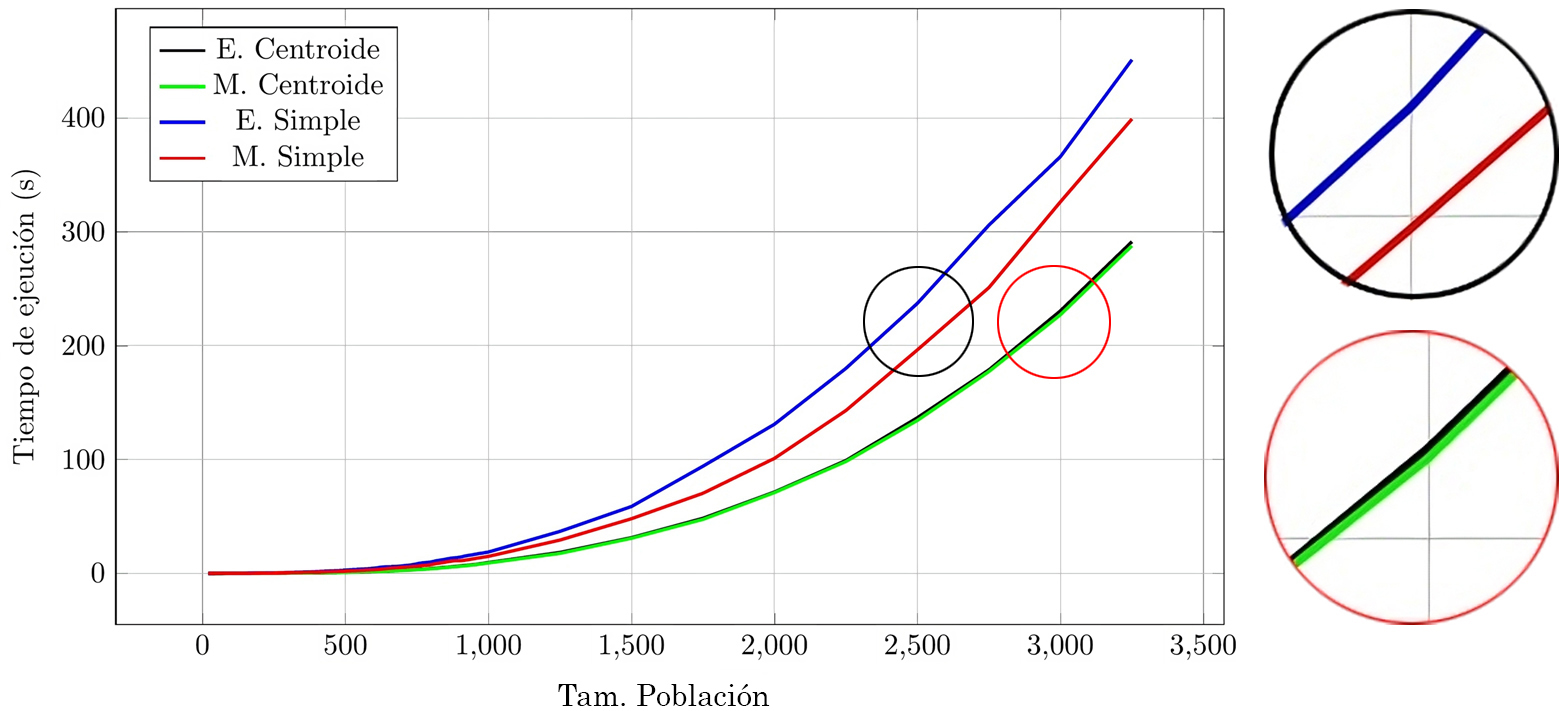
\includegraphics[width=\textwidth]{images/chapter_4/jerarquico}
	\caption{Tiempo de ejecución de las combinaciones de distancias en el algoritmo secuencial Jerárquico Aglomerativo}
	\label{fig:prueba_jerarquicosec}
\end{figure}





%\subsubsection{Distancia Centroide con mejoras}	
Una vez comprobado los tiempos de ejecución del algoritmo sin paralelizar, podemos pasar a las pruebas de las estrategias comentadas en la Sección \ref{cap:3_2_1}. Primero, estudiamos la distancia entre \textit{clusters} con menor tiempo de ejecución, por \textit{centroide}. Ejecutamos, con \textit{2}, \textit{4}, \textit{6} y \textit{8} procesos la primera estrategia en tres diferentes poblaciones. No aplicamos la segunda y tercera estrategia, pues estas están diseñadas para las distancias por enlace \textit{simple} y \textit{completo}.


La Figura \ref{fig:JA_centroide} muestra un buen rendimiento, reduciendo los tiempos de ejecución hasta con tamaños de poblaciones elevados. Para una población de \textit{5000} individuos se consiguen los siguientes \textit{speed-ups [1.78, 2.89, 3.61, 4.21]} utlizando \textit{2}, \textit{4}, \textit{6} y \textit{8} procesos, respectivamente. Los \textit{speed-ups} no crecen en proporción a los procesos ejecutados. La estrategia implementada, para tamaños de poblaciones elevados, no es óptima. Si un proceso no elimina filas en muchas iteraciones, acumula muchos más datos que procesar que los demás procesos, provocando que los procesos con menos datos esperen para seguir con la ejecución.

% JERARQUICO AGLOMERATIVO: HISTOGRAMA CON VARIOS PROCESOS
\begin{figure}[!h]
	\centering
	\begin{tikzpicture}
		\begin{axis}[
			ybar,
			bar width=0.35cm,
			ylabel={Tiempo de ejecución (s)},
			xlabel={Tam. Población},
			symbolic x coords={1000, 2500, 5000},
			xtick=data,
			enlarge x limits=0.2,
			ymin=0,
			width=\textwidth,
			height=0.45\textwidth,
			legend style={at={(0.5,1.13)}, anchor=north, legend columns=-1},
			area legend
			]
			
			\addplot+[ybar, pattern=vertical lines, draw=black] plot coordinates 
			{(1000, 7.61) (2500, 141.59) (5000, 1098.29)};
			\addplot+[ybar, pattern=grid, draw=black] plot coordinates 
			{(1000, 4.81) (2500, 79.61) (5000, 617.44)};
			\addplot+[ybar, pattern=dots, draw=black] plot coordinates 
			{(1000, 2.75) (2500, 47.36) (5000, 379.42) };
			\addplot+[ybar, pattern=crosshatch, draw=black] plot coordinates 
			{(1000, 2.24) (2500, 38.55) (5000, 304.12) };
			\addplot+[ybar, pattern=checkerboard, draw=black] plot coordinates 
			{(1000, 1.98) (2500, 33.13) (5000, 260.77)};
			
			
			\legend{Secuencial, MPI(2),MPI(4),MPI(6),MPI(8)}
		\end{axis}
	\end{tikzpicture}
	\caption{Tiempo de ejecución de la distancia entre \textit{clusters} por \textit{centroide} del algoritmo Jerárquico Aglomerativo en ordenador de propósito general}
	\label{fig:JA_centroide}
\end{figure}



%\subsubsection{Distancia por enlace Simple/Completo con mejoras}

Ahora veamos el comportamiento de las estrategias para la distancia entre \textit{clusters} con mayor complejidad, enlace \textit{simple} o \textit{completo}. Las pruebas se realizan con tamaños de poblaciones inferiores a las pruebas anteriores. Estos son los siguientes \textit{[100, 200, 500, 1000, 1500, 2000]}, y se ejecutan las estrategias con cuatro procesos para comprobar el rendimiento. La tercera estrategia tiene el mismo rendimiento que la segunda, pero con más procesos. Reservar procesos únicamente para el cálculo de nuevas distancias no es eficaz, es mejor dividir entre los procesos activos (segunda estrategia). La Figura \ref{fig:JA_simple} muestra los resultados obtenidos del estudio. Aunque sí reduce el tiempo de ejecución, no se obtienen buenos resultados, pues el \textit{speed-up} con \textit{2000} individuos de población para la estrategia con mejores resultados es de \textit{1.88}. Al usar cuatro procesos, podemos concluir que los tres \textit{workers} pierden mucho tiempo calculando las distancias en cada iteración. Es posible que, mediante la refinación progresiva de la segunda estrategia a través de un proceso iterativo de prueba y error, se logre reducir el tiempo de ejecución. No obstante, hasta el momento, no hemos logrado reducirlo más allá del tiempo actual.

\begin{figure}[!h]
	\hspace{-0.10\textwidth}
	\begin{tikzpicture}
		\begin{axis}[
			xlabel={Tam. Población},
			ylabel={Tiempo de ejecución (s)},
			legend style={at={(1.02,0.5)}, anchor=west},
			grid=major,
			width=\textwidth,
			height=0.45\textwidth,
			legend cell align={left},
			extra description/.code={
				\node at (1.01, 0.69) [anchor=west] {\textbf{Cores}};
			}
			]
			
			\addplot [mark=*, color=black, line width=1.2pt] table [x index=0, y index=1, col sep=space] {files/jerarquico_aglom_simple.txt};
			\addplot [mark=square*, color=red, line width=1.2pt] table [x index=0, y index=2, col sep=space] {files/jerarquico_aglom_simple.txt};
			\addplot [mark=triangle*, color=darkgreen, line width=1.2pt] table [x index=0, y index=3, col sep=space] {files/jerarquico_aglom_simple.txt};
			
			
			\addlegendentry{Secuencial}
			\addlegendentry{MPI\_1(4)}
			\addlegendentry{MPI\_2(4)}
			
			
		\end{axis}
	\end{tikzpicture}
	\caption{Tiempo de ejecución de la distancia entre \textit{clusters} por enlace \textit{simple} del algoritmo Jerárquico Aglomerativo en ordenador de propósito general}
	\label{fig:JA_simple}
\end{figure}


%\subsubsection{Cluster}	
Los resultados de la prueba anterior, con la complejidad del algoritmo indican que no es viable probar las estrategias implementadas sobre estas distancias entre \textit{cluster} en el sistema distribuido. Por este motivo, solo se prueba la distancia por \textit{centroides} con tres grandes poblaciones. Los tamaños son los siguientes \textit{[5000, 7500, 10000]}, y se prueban con \textit{20}, \textit{50}, \textit{75}, \textit{100} y \textit{128} procesos. La Figura \ref{fig:JA_cluster} muestra los resultados, y concluimos que para agrupar tamaños de poblaciones elevados no conviene aplicar este algoritmo. 


\begin{figure}[!h]
	\hspace{-0.07\textwidth}
	\begin{tikzpicture}
		\begin{axis}[
			xlabel={Tam. Población ($10^3$)},
			ylabel={Tiempo de ejecución (s)},
			xtick={5,7.5,10},
			legend style={at={(1.02,0.5)}, anchor=west},
			grid=major,
			width=\textwidth,
			height=0.45\textwidth,
			scaled x ticks=false,
			legend cell align={left},
			extra description/.code={
				\node at (1.01, 0.77) [anchor=west] {\textbf{Cores}};
			}
			]
			
			\addplot [mark=*, color=red, line width=1.2pt] table [x index=0, y index=1, col sep=space] {files/cluster/jerarquico_aglomerativo.txt};
			\addplot [mark=square*, color=magenta, line width=1.2pt] table [x index=0, y index=2, col sep=space] {files/cluster/jerarquico_aglomerativo.txt};
			\addplot [mark=triangle*, color=blue, line width=1.2pt] table [x index=0, y index=3, col sep=space] {files/cluster/jerarquico_aglomerativo.txt};
			\addplot [mark=star, color=orange, line width=1.2pt] table [x index=0, y index=4, col sep=space] {files/cluster/jerarquico_aglomerativo.txt};
			\addplot [mark=diamond*, color=darkgreen, line width=1.2pt] table [x index=0, y index=5, col sep=space] {files/cluster/jerarquico_aglomerativo.txt};
			%\addplot [mark=otimes*, color=cyan, line width=1.2pt] table [x index=0, y index=6, col sep=space] {files/cluster/kmedias5D.txt};
			%\addplot [mark=triangle*, color=darkgreen, line width=1.2pt] table [x index=0, y index=7, col sep=space] {files/cluster/kmedias5D.txt};
			
			\addlegendentry{20}
			\addlegendentry{50}
			\addlegendentry{75}
			\addlegendentry{100}
			\addlegendentry{128}
			
		\end{axis}
	\end{tikzpicture}
	\caption{Tiempo de ejecución de la distancia entre \textit{clusters} por \textit{centroide} del algoritmo Jerárquico Aglomerativo en Cluster}
	\label{fig:JA_cluster}
\end{figure}


O por lo menos las estrategias implementadas no dan resultados notorios, pues el \textit{speed-up} entre usar \textit{20} o \textit{128} procesos en una población de \textit{10000} individuos es de \textit{2.32}.

% ------------------------------------------------------------------------------------------------
% --- KMEDIAS ------------------------------------------------------------------------------------
% ------------------------------------------------------------------------------------------------


\subsection{K-Medias}	

El algoritmo anterior no tiene ninguna variable que modifique el tiempo de ejecución (sin contar la distancia entre clusters). Esta técnica de agrupación tiene un coste temporal mucho menor que el aglomerativo, \textit{O(N*K*iter)} siendo \textit{N} el tamaño de la población, \textit{iter} las iteraciones hasta que no cambien los centros y \textit{K} el número de centros. \textit{(N $\gg$ K,iter)} \textit{K} e \textit{iter} no son valores muy altos, por lo que la complejidad no llega a ser cuadrática. Cuanto mayor sea el valor de \textit{K}, más tiempo va a consumir para realizar la asignación, pues cada individuo de la población es comparado con más centros. No obstante, dependiendo de la asignación de los individuos,  una ejecución con más centros puede ser más rápida que otra con menos centros. Todo depende de la variable \textit{iter}, es decir, si consigue llegar antes a la condición de finalización (que los centros no cambien entre dos iteraciones). La Figura \ref{fig:Kmedias_variarK} muestra precisamente este punto. Para dos poblaciones distintas, de \textit{75000} y \textit{100000} individuos aplicando \textit{K=25} centros (línea roja), requieren aproximadamente el mismo tiempo. La primera población itera muchas veces, más en concreto, el doble de veces que la segunda población para finalizar la ejecución. Una ejecución del algoritmo sobre una misma población puede variar considerablemente dependiendo del número de centros, o la disposición de los mismos.



\begin{figure}[!h]
	\centering
	\begin{tikzpicture}
		\begin{axis}[
			width=0.85\textwidth,
			height=0.40\textwidth,
			ybar,
			bar width=0.35cm,
			ylabel={Tiempo de ejecución (s)},
			xlabel={Tam. de la Población},
			symbolic x coords={25000, 50000, 75000, 100000},
			xtick=data,
			enlarge x limits=0.2,
			ymin=0,
			legend style={at={(0.5,1.13)}, anchor=north, legend columns=-1},
			extra description/.code={
				\node at (0.28, 1.12) [anchor=north] {\textbf{K}};
			},
			area legend,
			legend columns=4,					
			]
			
			% Histo
			\addplot+[ybar, pattern=vertical lines, draw=black] plot coordinates 
			{(25000, 0.62) (50000, 1.31) (75000, 1.66) (100000, 2.56)};				
			\addplot+[ybar, pattern=grid, draw=black] plot coordinates 
			{(25000, 1.69) (50000, 4.22) (75000, 5.19)  (100000, 8.76)};						
			\addplot+[ybar, pattern=dots, draw=black] plot coordinates 
			{(25000, 8.29) (50000, 33.80) (75000, 79.83) (100000, 79.56)};						
			\addplot+[ybar, pattern=crosshatch, draw=black] plot coordinates 
			{(25000, 19.93) (50000, 56.03) (75000, 109.96) (100000, 123.16)};
			
			\addlegendentry{5}
			\addlegendentry{10}
			\addlegendentry{25}
			\addlegendentry{50}
			
		\end{axis}
		
		\begin{axis}[
			width=0.85\textwidth,
			height=0.40\textwidth,
			axis y line=none,
			axis x line=none,
			ymin=0,				
			legend style={at={(1.02,0.5)}, anchor=west},
			legend cell align={left},
			extra description/.code={
				\node at (1.04, 0.82) [anchor=north] {\textbf{K}};
			}									
			]
			
			\addplot[smooth, mark=diamond, green] plot coordinates
			{(25000, 0.62) (50000, 1.31) (75000, 1.66) (100000, 2.56)};
			\addplot[smooth, mark=diamond, blue] plot coordinates
			{(25000, 1.69) (50000, 4.22) (75000, 5.19)  (100000, 8.76)};
			\addplot[smooth, mark=diamond, red] plot coordinates
			{(25000, 8.29) (50000, 33.80) (75000, 79.83) (100000, 79.56)};
			\addplot[smooth, mark=diamond, black] plot coordinates
			{(25000, 19.93) (50000, 56.03) (75000, 109.96) (100000, 123.16)};
			
			\addlegendentry{5}
			\addlegendentry{10}
			\addlegendentry{25}
			\addlegendentry{50}
			
		\end{axis}
	\end{tikzpicture}
	\caption{Variaciones en el número de \textit{clusters} (K) en el algoritmo K-Medias}
	\label{fig:Kmedias_variarK}
\end{figure}




%\subsubsection{Ordenador de propósito general}	

Las distancias entre individuos siguen presentes, pero esta vez, al tener una complejidad menor, no debería afectar tanto usar la distancia \textit{Euclídea} o \textit{Manhattan}. O eso es lo que parece a simple vista. Como se comprobó en la Figura \ref{fig:Kmedias_variarK}, el número de iteraciones para llegar a la condición de finalización importa, y usar una distancia u otra va a influir en el tiempo de ejecución. El número de iteraciones varía dependiendo de qué distancia se use, pues la \textit{Euclídea}, aunque su cálculo es más lento, tiene una mayor precisión, lo que le da una gran ventaja frente a la distancia \textit{Manhattan}. Esta última, al no ser tan precisa, puede hacer que, aunque sea por poco, un individuo pertenezca a otro \textit{cluster}, provocando una reacción en cadena que resulte en un aumento considerable en el número de iteraciones. 

El estudio realizado para comprobar el rendimiento de la estrategia comentada en la Sección \ref{cap:3_2_2} con cinco procesos frente el algoritmo secuencial, se representa en la Figura \ref{fig:KMedias}, utilizando \textit{K=10} centros, y comparando también las distancias entre individuos (\textit{Euclídea} y \textit{Manhattan}). Los tamaños de las poblaciones utilizadas para medir estas pruebas se realizan como en las pruebas de las ordenaciones cuadráticas (ver Sección \ref{cap:4_2_1_1}). Se puede apreciar que las funciones tienen picos, siendo más pronunciados en los algoritmos sin paralelizar. Como se comentó anteriormente, el tiempo de ejecución para una población puede variar dependiendo de la distancia implementada, además de la posibilidad de que una población con menor tamaño pueda tardar mucho más que una población mayor, debido a la disposición de los individuos y los \textit{clusters} en la ejecución. 						


\begin{figure}[!h]
	\centering
	\begin{tikzpicture}
		\begin{axis}[
			xlabel={Tam. Población ($10^4$)},
			ylabel={Tiempo de ejeución (s)},
			xtick={0,1,2,3,4,5,6,7,8,9,10},
			legend pos=north west,
			grid=major,
			width=\textwidth,
			height=0.4\textwidth,
			scaled x ticks=false,
			]
			
			
			\addplot [mark=none, color=blue, line width=1.2pt] table [x index=0, y index=1, col sep=space] {files/kmedias.txt};
			\addplot [mark=none, color=red, line width=1.2pt] table [x index=0, y index=2, col sep=space] {files/kmedias.txt};
			\addplot [mark=none, color=black, line width=1.2pt] table [x index=0, y index=3, col sep=space] {files/kmedias.txt};
			\addplot [mark=none, color=darkgreen, line width=1.2pt] table [x index=0, y index=4, col sep=space] {files/kmedias.txt};
			
			
			\addlegendentry{Euclídea}
			\addlegendentry{Manhattan}
			\addlegendentry{Euclídea\_MPI(5)}
			\addlegendentry{Manhattan\_MPI(5)}
			
			
		\end{axis}
	\end{tikzpicture}
	\caption{Tiempo de ejecución -con 5 procesos- de la primera estrategia del algoritmo K-Medias en ordenador de propósito general}
	\label{fig:KMedias}
\end{figure}


Comparando el algoritmo secuencial y el paralelizado se puede apreciar una mejora considerable, y debido a los picos, es interesante medir la evolución de los \textit{speed-ups}. La Figura \ref{fig:Kmedias_speedup} muestra esta evolución, cuyos \textit{speed-ups} son calculados con los tiempos utilizados en la anterior figura. Ambas distancias comienzan siendo volátiles, siendo algunas veces peor que el algoritmo secuencial (\textit{speed-up<1}) y otras veces superando por mucho el \textit{speed-up} ideal. A partir de diez mil individuos de población, el \textit{speed-up} es equivalente al número de \textit{workers} ejecutados. Tras analizar los resultados, observamos que, pese a que la distancia \textit{Euclídea} es más precisa, a la larga es mejor aplicar distancia \textit{Manhattan}, pues, aunque itere más veces, el coste es menor, llevando a conseguir mejores resultados. Se puede apreciar la línea azul superando en la mayoría de las veces a la línea roja, probando lo comentado.




\begin{figure}[!h]
	\centering
	\begin{tikzpicture}
		\begin{axis}[
			xlabel={Tam. Población ($10^4$)},
			ylabel={speed-up},
			xtick={0,1,2,3,4,5,6,7,8,9,10},
			legend pos=north east,
			grid=major,
			width=0.85\textwidth,
			height=0.40\textwidth,
			scaled x ticks=false,
			]
			
			
			\addplot [mark=none, color=darkgreen, line width=1.7pt] table [x index=0, y index=1, col sep=space] {files/kmedias_speedup.txt};
			\addplot [mark=none, color=red, line width=0.3pt] table [x index=0, y index=2, col sep=space] {files/kmedias_speedup.txt};
			\addplot [mark=none, color=blue, line width=0.3pt] table [x index=0, y index=3, col sep=space] {files/kmedias_speedup.txt};
			
			
			\addlegendentry{Ideal}
			\addlegendentry{Euclídea}
			\addlegendentry{Manhttan}
			
			
		\end{axis}
	\end{tikzpicture}
	\caption{Speed-up de la primera estrategia del algoritmo K-Medias en ordenador de propósito general usando 5 procesos}
	\label{fig:Kmedias_speedup}
\end{figure}



%\subsubsection{Cluster}

Para este algoritmo, al contrario que el anterior, se pueden realizar pruebas con tamaños de poblaciones mayores en el sistema distribuido. La siguiente prueba realizada comienza con una población de \textit{20000} individuos, esta vez con cinco variables de entrada. Entre pruebas se aumenta ese mismo tamaño hasta llegar a \textit{240000} individuos, utilizando en proporción una población seis veces mayor que en el ordenador de propósito general. Se usa el mismo valor de \textit{K} (\textit{K=10}), y se ejecuta la misma estrategia con \textit{10}, \textit{20}, \textit{35}, \textit{50}, \textit{75}, \textit{100} y \textit{128} procesos. Como se muestra en la Figura \ref{fig:Kmedias_cluster}, a partir de veinte procesos, la reducción del tiempo de ejecución se ralentiza. Con un número elevado de procesos, esta estrategia no consigue reducir el tiempo de ejecución en proporción a los procesos ejecutados, esto se debe a la gran cantidad de comunicaciones que se deben realizar para finalizar la ejecución.


\begin{figure}[!h]
	\hspace{-0.07\textwidth}
	\begin{tikzpicture}
		\begin{axis}[
			xlabel={Tam. Población ($10^4$)},
			ylabel={Tiempo de ejecución (s)},
			xtick={2,4,6,8,10,12,14,16,18,20,22,24},
			legend style={at={(1.02,0.5)}, anchor=west},
			grid=major,
			width=\textwidth,
			height=0.45\textwidth,
			scaled x ticks=false,
			legend cell align={left},
			extra description/.code={
				\node at (1.01, 0.85) [anchor=west] {\textbf{Cores}};
			}
			]
			
			\addplot [mark=*, color=red, line width=1.2pt] table [x index=0, y index=1, col sep=space] {files/cluster/kmedias5D.txt};
			\addplot [mark=square*, color=magenta, line width=1.2pt] table [x index=0, y index=2, col sep=space] {files/cluster/kmedias5D.txt};
			\addplot [mark=triangle*, color=blue, line width=1.2pt] table [x index=0, y index=3, col sep=space] {files/cluster/kmedias5D.txt};
			\addplot [mark=star, color=orange, line width=1.2pt] table [x index=0, y index=4, col sep=space] {files/cluster/kmedias5D.txt};
			\addplot [mark=diamond*, color=purple, line width=1.2pt] table [x index=0, y index=5, col sep=space] {files/cluster/kmedias5D.txt};
			\addplot [mark=otimes*, color=cyan, line width=1.2pt] table [x index=0, y index=6, col sep=space] {files/cluster/kmedias5D.txt};
			\addplot [mark=triangle*, color=darkgreen, line width=1.2pt] table [x index=0, y index=7, col sep=space] {files/cluster/kmedias5D.txt};
			
			\addlegendentry{10}
			\addlegendentry{20}
			\addlegendentry{35}
			\addlegendentry{50}
			\addlegendentry{75}
			\addlegendentry{100}
			\addlegendentry{128}
			
		\end{axis}
	\end{tikzpicture}
	\caption{Tiempo de ejecución de la primera estrategia del algoritmo K-Medias en el Cluster}
	\label{fig:Kmedias_cluster}
\end{figure}



\begin{comment}	
	
	Ahora bien, veamos la 
	
	
	\newpage
	
	\begin{figure}[!h]
		\centering
		\begin{tikzpicture}
			\begin{axis}[
				xlabel={Tam. Población ($10^4$)},
				ylabel={Tiempo de ejecución (s)},
				xtick={2,4,6,8,10,12,14,16,18,20,22,24},
				legend style={at={(1.02,0.5)}, anchor=west},
				grid=major,
				width=\textwidth,
				height=0.45\textwidth,
				scaled x ticks=false,
				legend cell align={left},
				extra description/.code={
					\node at (1.01, 0.72) [anchor=west] {\textbf{Cores}};
				}
				]
				
				\addplot [mark=*, color=black, line width=1.2pt] table [x index=0, y index=1, col sep=space] {files/cluster/kmediasDs.txt};
				\addplot [mark=square*, color=red, line width=1.2pt] table [x index=0, y index=2, col sep=space] {files/cluster/kmediasDs.txt};
				\addplot [mark=triangle*, color=darkgreen, line width=1.2pt] table [x index=0, y index=3, col sep=space] {files/cluster/kmediasDs.txt};
				\addplot [mark=star, color=blue, line width=1.2pt] table [x index=0, y index=4, col sep=space] {files/cluster/kmediasDs.txt};
				
				
				\addlegendentry{50\_2D}
				\addlegendentry{50\_5D}
				\addlegendentry{100\_2D}
				\addlegendentry{100\_5D}
				
			\end{axis}
		\end{tikzpicture}
		\caption{KMedias - Diferencia de dimensiones calculada en el cluster}
	\end{figure}
	
	La diferencia entre usar más dimensiones en este algoritmo es abismal, llegando a ser cinco veces más lento tener una población tan elevada, con tres dimensiones (variables) más. Esto se debe a que el algoritmo está constantemente calculando distancias, lo que provoca, aplicando distancia euclidea, una diferencia significativa.
\end{comment}



% ------------------------------------------------------------------------------------------------
% --- KNN ----------------------------------------------------------------------------------------
% ------------------------------------------------------------------------------------------------		
\subsection{KNN}


En cada iteración de este algoritmo de aprendizaje supervisado, se clasifica un individuo utilizando una población previamente categorizada. Al contrario que los algoritmos de aprendizaje no supervisado, que agrupan una población entera al finalizar la población. La complejidad temporal de este algoritmo es menor, y el valor de \textit{K} no influye en el tiempo de ejecución como el algoritmo de \textit{K-Medias}, pues al aumentar este valor solo aumenta el número de los individuos más cercanos que se comprueban para categorizar el nuevo individuo. Este algoritmo usa dos poblaciones, y como se comentó en la Sección \ref{cap:3_2_3}, las dos estrategias dividen una de las poblaciones para paralelizar el algoritmo. 

Para las siguientes pruebas realizadas en el ordenador de propósito general, se fija la misma población utilizada en el algoritmo anterior, con un tamaño de \textit{100000} individuos para la población a categorizar. La población inicialmente categorizada tiene un tamaño de mil individuos y se obtiene realizando una búsqueda exhaustiva con el algoritmo K-Medias. Esta búsqueda se realiza con valores de K en el intervalo de [\textit{2, 20]} centros, ejecutando, para cada uno, el algoritmo diez veces, calculando así la mejor agrupación. Se obtiene como resultado cuatro centros. Con estas dos poblaciones se ejecuta el algoritmo de \textit{K-Vecinos más Cercanos} con un valor de \textit{K=15}, un número impar para que no haya posibilidad de empates a la hora de asignar un \textit{cluster} a cada individuo.

%\subsubsection{Algoritmo sin mejoras}

Primero comprobamos los dos métodos para el algoritmo secuencial, actualizar o no actualizar al categorizar un nuevo individuo. Si se actualiza la población conforme avanzan las iteraciones, la población final será mucho más precisa que si no se actualiza, pero el tiempo de ejecución aumentará considerablemente. La Figura \ref{fig:knn_secuencial} muestra los resultados. Si no se actualiza, la complejidad es lineal, pues la población categorizada se mantiene constante, y no se puede diferenciar cuál de las dos distancias ralentiza más la ejecución. Sin embargo, cuando se actualiza la población, se comprueba una vez más que la distancia \textit{Euclídea} es más lenta que la \textit{Manhattan}.


% KNN BASICO
\begin{figure}[!h]
	\centering
	\begin{tikzpicture}
		\begin{axis}[
			xlabel={Tam. Población ($10^4$)},
			ylabel={Tiempo de ejeución (s)},
			xtick={0,1,2,3,4,5,6,7,8,9,10},
			legend pos=north west,
			legend columns=2,
			grid=major,
			width=\textwidth,
			height=0.45\textwidth,
			scaled x ticks=false,
			]
			
			
			\addplot [mark=none, color=darkgreen, line width=1.2pt] table [x index=0, y index=1, col sep=space] {files/knn.txt};
			\addplot [mark=none, color=red, line width=1.2pt] table [x index=0, y index=3, col sep=space] {files/knn.txt};
			\addplot [mark=none, color=black, line width=1.2pt] table [x index=0, y index=2, col sep=space] {files/knn.txt};
			
			\addplot [mark=none, color=blue, line width=1.2pt] table [x index=0, y index=4, col sep=space] {files/knn.txt};
			
			
			\addlegendentry{Euclídea}
			\addlegendentry{Euclídea\_Act}
			\addlegendentry{Manhattan}
			
			\addlegendentry{Manhattan\_Act}
			
			
		\end{axis}
	\end{tikzpicture}
	\caption{Tiempo de ejecución del algoritmo secuencial KNN en ordenador de propósito general}
	\label{fig:knn_secuencial}
\end{figure}



%\subsubsection{Algoritmo con mejoras}
Después de comprobar el algoritmo secuencial pasamos a las estrategias para reducir el tiempo de ejecución. El algoritmo sin actualizar es rápido y es mejor estudiar el comportamiento con una población variable con el tiempo. Por eso se ejecutan las dos estrategias con cinco procesos. Podemos ver los resultados en la figura \ref{fig:knn_ordenador}, con una reducción notoria en el tiempo de ejecución. Para la primera estrategia, dividir la población categorizada entre los \textit{workers}, se realizan dos versiones, una en la que cada \textit{worker} espera el individuo categorizado de la iteración anterior (línea de color verde), y otra en la que no se espera, sino que los \textit{workers} trabajan en la siguiente iteración mientras que el \textit{master} agrupa el individuo (línea de color negro). La primera estrategia es ligeramente más rápida que la segunda (línea de color azul), y aun perdiendo tiempo esperando a la categorización del individuo (la primera versión), sigue finalizando antes que la segunda estrategia. 

En cuestión de complejidad espacial la segunda estrategia consume mucha más memoria. Al finalizar la ejecución, cada \textit{worker} tiene una copia entera de la población categorizada, mientras que en la primera mejora se divide esta población entre los procesos. 


\begin{figure}[!h]
	\centering
	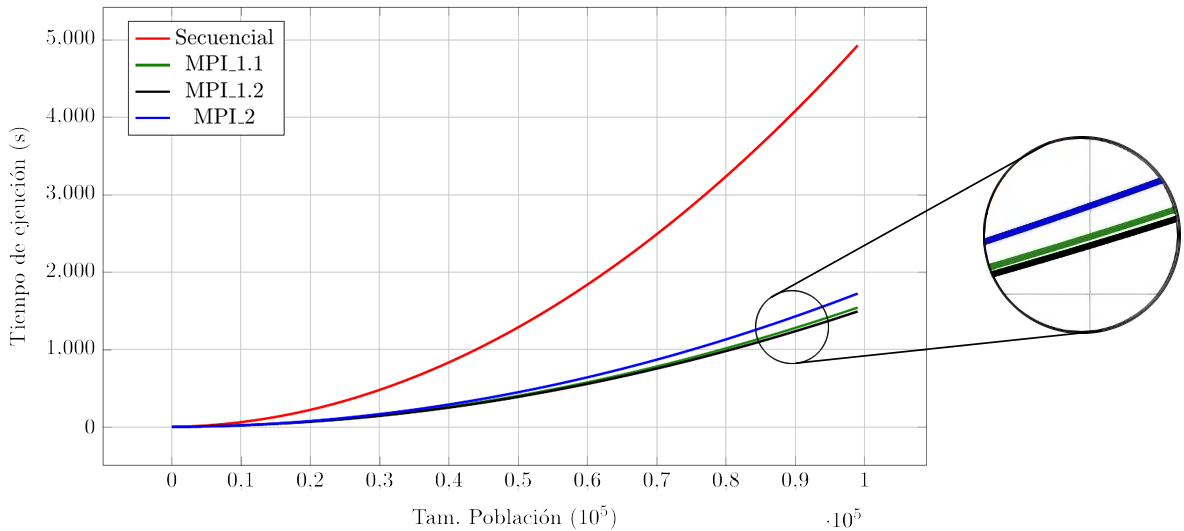
\includegraphics[width=1\textwidth]{images/chapter_4/knn_mpi}
	\caption{Tiempo de las estrategias del algoritmo KNN en ordenador de propósito general}
	\label{fig:knn_ordenador}
\end{figure}


Comparando las evoluciones de los \textit{speed-ups} en las estrategias, se puede concluir que al principio es mejor dividir la población a predecir, pero a largo plazo es más efectivo dividir la población categorizada, además de tener menos complejidad espacial. 

\begin{figure} [!h]
	\centering
	\begin{tikzpicture}
		\begin{axis}[
			xlabel={Tam. Población ($10^4$)},
			ylabel={speed-up},
			xtick={0,1,2,3,4,5,6,7,8,9,10},
			legend pos=south east,			
			legend columns=3,
			grid=major,
			width=1\textwidth,
			height=0.35\textwidth,
			scaled x ticks=false,
			]
			
			\addplot [mark=none, color=darkgreen, line width=0.8pt] table [x index=0, y index=1, col sep=space] {files/knn_speedup.txt};
			\addplot [mark=none, color=red, line width=0.8pt] table [x index=0, y index=2, col sep=space] {files/knn_speedup.txt};
			\addplot [mark=none, color=blue, line width=0.8pt] table [x index=0, y index=3, col sep=space] {files/knn_speedup.txt};
			
			
			\addlegendentry{Ideal}
			\addlegendentry{MPI\_1}
			\addlegendentry{MPI\_2}
			
			
		\end{axis}
	\end{tikzpicture}
	\caption{\textit{Speed-ups} de las estrategias del algoritmo KNN en ordenador de propósito general}
\end{figure}


%\subsubsection{Cluster}

En algoritmos pasados ya hemos visto el funcionamiento de varias estrategias con tamaños de poblaciones elevados. Esta vez, para las pruebas en el sistema distribuido, ejecutamos la misma prueba que antes, pero con más procesos en paralelo. Se ejecutan \textit{10}, \textit{20}, \textit{35}, \textit{50}, \textit{75}, \textit{100} y \textit{128} procesos sobre la mejor estrategia obtenida en el estudio anterior, comprobar el \textit{speed-up} al usar muchos procesos. La Figura \ref{fig:knn_cluster} muestra que, al aumentar los procesos, no se reduce considerablemente el tiempo de ejecución, generando sobrecarga a partir de veinte procesos. Al igual que en el algoritmo \textit{K-Medias}, aumentar el número de procesos provoca que, aunque se reduce el tiempo de ejecución en cada iteración, el tiempo de comunicación (overhead) entre iteraciones aumenta. 




\begin{figure}[!h]
	\hspace{-0.07\textwidth}
	\begin{tikzpicture}
		\begin{axis}[
			xlabel={Tam. Población ($10^4$)},
			ylabel={Tiempo de ejecución (s)},
			legend style={at={(1.02,0.5)}, anchor=west},
			grid=major,
			width=\textwidth,
			height=0.45\textwidth,
			scaled x ticks=false,
			legend cell align={left},
			extra description/.code={
				\node at (1.01, 0.85) [anchor=west] {\textbf{Cores}};
			}
			]
			
			\addplot [mark=, color=red, line width=1.2pt] table [x index=0, y index=1, col sep=space] {files/cluster/knn.txt};
			\addplot [mark=, color=magenta, line width=1.2pt] table [x index=0, y index=2, col sep=space] {files/cluster/knn.txt};
			\addplot [mark=, color=blue, line width=1.2pt] table [x index=0, y index=3, col sep=space] {files/cluster/knn.txt};
			\addplot [mark=, color=orange, line width=1.2pt] table [x index=0, y index=4, col sep=space] {files/cluster/knn.txt};
			\addplot [mark=, color=black, line width=1.2pt] table [x index=0, y index=5, col sep=space] {files/cluster/knn.txt};
			\addplot [mark=, color=cyan, line width=1.2pt] table [x index=0, y index=6, col sep=space] {files/cluster/knn.txt};
			\addplot [mark=, color=darkgreen, line width=1.2pt] table [x index=0, y index=7, col sep=space] {files/cluster/knn.txt};
			
			
			
			\addlegendentry{10}
			\addlegendentry{20}
			\addlegendentry{35}
			\addlegendentry{50}
			\addlegendentry{75}
			\addlegendentry{100}
			\addlegendentry{128}
			
		\end{axis}
	\end{tikzpicture}
	\caption{Tiempo de la primera estrategia del algoritmo KNN en Cluster}
	\label{fig:knn_cluster}
\end{figure} 



% ------------------------------------------------------------------------------------------------
% --- RL -----------------------------------------------------------------------------------------
% ------------------------------------------------------------------------------------------------

\section{Q-Learning}	

Para el aprendizaje por refuerzo, cuyos dos algoritmos se comentaron en la Sección \ref{cap:2_2}, primero se estudia el algoritmo de \textit{Q-Learning}. El otro algoritmo, \textit{Deep Q-Network}, se basa en redes neuronales, estudio que se realiza posteriormente en la Sección \ref{cap:4_6}.


%\subsubsection{Algoritmo sin mejoras}
Antes de entrar en profundidad con las estrategias comentadas en la Sección \ref{cap:3_3}, primero estudiamos el comportamiento del algoritmo de manera secuencial, con y sin preprocesado del entorno. Este preprocesado consiste en recorrer la matriz entera eliminando estados inaccesibles (el agente se sitúa en un muro) y acciones que no queremos que el agente ejecute, como chocar con una pared. Se ejecuta con tres laberintos diferentes, con \textit{30}, \textit{50} y \textit{100} filas. La Figura \ref{fig:rl_preprocesado} muestra una leve reducción en el tiempo de ejecución. Además, obtiene mejores resultados con una mayor variedad de combinaciones de hiper-parámetros. Al reducir las acciones disponibles, el agente tiene una mayor probabilidad de explorar más el laberinto, generando más combinaciones con las cuales aprender el camino óptimo hasta la meta.			


\begin{figure}[!h]
	\centering
	\begin{tikzpicture}
		\begin{axis}[
			xlabel={Tam. del Laberinto},
			ylabel={Tiempo de ejeución (s)},
			xtick={30,50,100},
			legend pos=north west,
			grid=major,
			width=\textwidth,
			height=0.35\textwidth
			]
			
			
			\addplot [mark=none, color=red, line width=1.2pt] table [x index=0, y index=1, col sep=space] {files/rl.txt};
			\addplot [mark=none, color=darkgreen, line width=1.2pt] table [x index=0, y index=2, col sep=space] {files/rl.txt};
			
			
			\addlegendentry{Normal}
			\addlegendentry{Preprocesado}
			
			
		\end{axis}
	\end{tikzpicture}
	\caption{Tiempo de ejecución del algoritmo secuencial Aprendizaje por Refuerzo en ordenador de propósito general}
	\label{fig:rl_preprocesado}
\end{figure}



%\subsubsection{Búsqueda de los mejores hiper-parámetros}

Una buena configuración de hiper-parámetros genera que el agente logre alcanzar su objetivo. En entornos de gran tamaño, algunas veces, es complicado encontrar configuraciones que funcionen, lo que provoca un aumento en el tiempo dedicado a la fase de entrenamiento para encontrar estas combinaciones. Por este motivo, se desarrolla una estrategia para encontrar combinaciones de los hiper-parámetros realizando una búsqueda exhaustiva. 

Consiste en ejecutar en muchos procesos el algoritmo secuencial sin preprocesar con diferentes combinaciones. Se inicializa \textit{100} filas y columnas, y con una precisión de \textit{0.01}, es decir un \textit{1\%}, el \textit{master} aumenta los valores de los hiper-parámetros. Cuando uno de estos llega al \textit{100\%} se reinicia y aumenta el siguiente, así hasta cubrir todas las posibles combinaciones. Al ser tres hiper-parámetros hay \(10^{6}\) combinaciones distintas. El \textit{master} envía a cada \textit{worker} diferentes combinaciones, y cuando terminan de procesar una combinación, envían de vuelta un mensaje de confirmación. Si termina con éxito, el \textit{master} almacena en un fichero la combinación de hiper-parámetros, junto con los movimientos requeridos, así como las veces que el algoritmo falla y llega a la meta. En caso contrario no almacena nada. Dicha prueba se realizó en el sistema distribuido, con \textit{128} procesos, y ha tardado siete días completos en finalizar la prueba, obteniendo \textit{500} combinaciones distintas, de las cuales, solo la mitad dan con el camino óptimo.






%\subsubsection{Mejora: Ejecuciones en paralelo}
Una vez estudiado las combinaciones de hiper-parámetros, podemos pasar a las pruebas de las estrategias para reducir el tiempo de ejecución del algoritmo. Para ello, se usa un laberinto de cien filas y columnas, con una combinación de hiper-parámetros que sea óptima (alguna de las previamente encontradas). El algoritmo secuencial ejecuta \textit{100} episodios (iteraciones que finalizan al llegar a la meta), mientras que la estrategia paralelizada, ejecuta, con cinco procesos, \textit{400} episodios. Esta estrategia, usando el modelo \textit{Master-Worker} se basa en la misma idea de encontrar las combinaciones de hiper-parámetros, pues se ejecuta en paralelo el algoritmo secuencial, pero esta vez en diferentes posiciones. Al final de la ejecución, el \textit{master} realiza la media de las experiencias obtenidas en todo el entorno. 

La imagen a la izquierda de la Figura \ref{fig:RL_estrategia1} muestra el mapa de calor del algoritmo secuencial y la estrategia. En rojo se representan las celdas que más veces han sido visitadas por el algoritmo secuencial, mientras que en verde las del paralelizado. En amarillo se representan los puntos de salida, siendo el superior izquierdo el del algoritmo secuencial y un proceso \textit{worker} de la estrategia paralelizada (para la estrategia paralelizada hay que garantizar que haya al menos un proceso en el punto origen). Para obtener este mapa se hacen unas comparaciones de las celdas visitadas, haciendo la media en el caso de la estrategia, pues sin hacerla se obtendría una mapa completamente verde. Se puede observar que el algoritmo secuencial visita más veces la parte superior izquierda, debido a que la media de veces que se visita esa zona en la estrategia se divide entre cuatro, y al ser menos probable que todos los \textit{workers} la visiten, hace que la ejecución secuencial la visite más veces, ya que siempre se inicializa por esa zona. 

Los tiempos de ejecución son similares. El tiempo de ejecución de la estrategia paralelizada viene dada por el mayor tiempo de ejecución de los \textit{workers}. El \textit{worker} que más tiempo consume es el que está posicionado en la misma salida que el algoritmo secuencial, por lo que por la aleatoriedad y el tiempo de comunicación con el proceso \textit{master} provoca que la ejecución total de la estrategia sea más lenta. No obstante, esta estrategia visita muchas más celdas en el laberinto, además de ejecutar cuatro veces más episodios sumando los ejecutados en cada proceso.		

\begin{figure}[!h]
	\centering
	\begin{subfigure}[t]{0.4\textwidth}
		\centering
		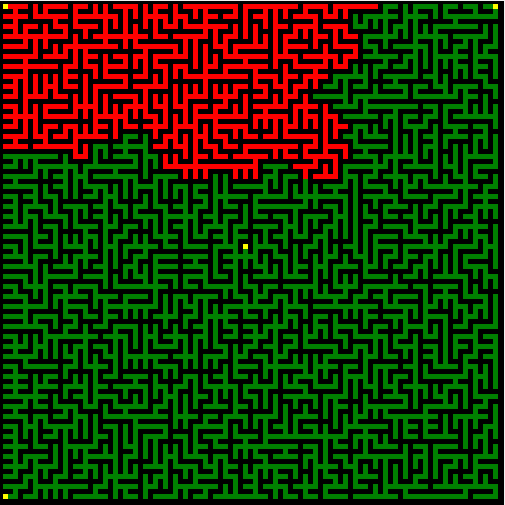
\includegraphics[width=\textwidth]{images/chapter_4/mapa_calor}
		\caption{Mapa de calor del laberinto \textit{100x100}}
		\label{fig:RL_mapa_calor}
	\end{subfigure}
	\hfill
	\begin{subfigure}[t]{0.5\textwidth}
		\centering
		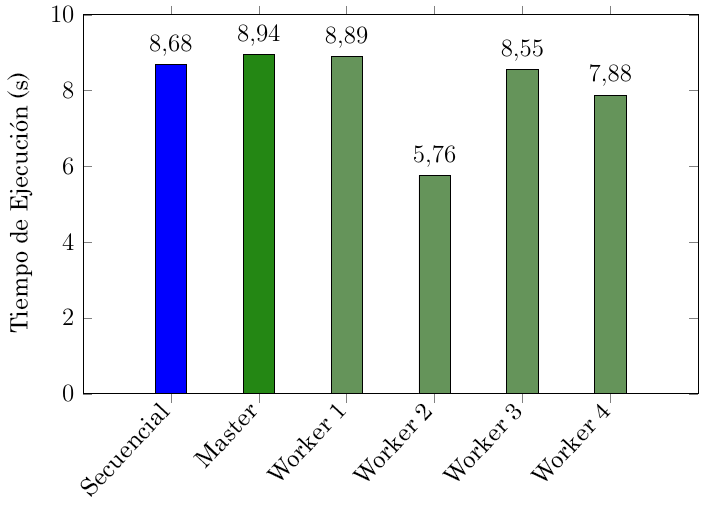
\includegraphics[width=\textwidth]{images/chapter_4/histo}
		\caption{Procesos y modo de ejecución}
		\label{fig:RL_histo}
	\end{subfigure}
	\caption{Tiempo de ejecución y mapa de calor de la primera estrategia del algoritmo Aprendizaje por Refuerzo en ordenador de propósito general}
	\label{fig:RL_estrategia1}
\end{figure}


La segunda estrategia, dividir el entorno entre los procesos ejecutados, no funciona correctamente. En la fase de entrenamiento no se ha conseguido finalizar, en ninguna de las pruebas realizadas, en una matriz de treinta filas y columnas (el laberinto de menor tamaño generado previamente). No obstante, al ejecutar la estrategia con valores aprendidos en un entrenamiento secuencial, sí se logra llegar a la meta. Hemos comprobado con varios hiper-parámetros y ninguno termina el entrenamiento. La teoría más razonable es que esta estrategia está muy influenciada por la combinación de hiper-parámetros, provocando que una mala configuración lleve a un mal aprendizaje, generando bucles infinitos.








% ------------------------------------------------------------------------------------------------
% --- PEV ----------------------------------------------------------------------------------------
% ------------------------------------------------------------------------------------------------	
\section{Algoritmos Evolutivos}

Este algoritmo no se ejecuta sobre unos datos previamente generados, sino que en cada ejecución crea desde cero los individuos que van a evolucionar para optimizar una función de evaluación. Las pruebas realizadas en esta sección en el ordenador de propósito general se ejecutan sobre los siguientes tamaños de poblaciones \textit{[25, 50, 100, 200, 500, 1000, 2000]} con \textit{100} generaciones. Para garantizar la supervivencia de los mejores individuos se utiliza un 5\% de elitismo. 

Como cada individuo tiene su propia estructura, no se puede aplicar los mismos métodos para las partes del algoritmo. El cruce y la mutación varían dependiendo del individuo, pero se eligen los más básicos. La selección es común para todos los individuos. Debido a que solo juega con los valores \textit{fitness} (aptitud del individuo para resolver el problema) calculados en las funciones de evaluación, que se comentaron en la Sección \ref{cap:3_4}. Esta selección consiste en elegir aleatoriamente los individuos, cuyas probabilidades de selección aumentan o disminuyen dependiendo de su valor de \textit{fitness}. Para la función de evaluación, además de contar con el cálculo del \textit{fitness}, también cuenta con otras funcionalidades como el desplazamiento de individuos, que consiste en garantizar que todos tengan un valor \textit{fitness} positivo, además de controlar la diversidad con un escalado lineal. Para los individuos representados como árboles, se añade un control de \textit{bloating}, controlando así la altura de los individuos, generando un leve aumento en el tiempo de la función de evaluación, pues si un individuo supera un límite de altura en el árbol, se sustituye con uno nuevo generado de manera aleatoria. Las complejidades del cálculo \textit{fitness} y las variables que afectan a los tamaños de las pruebas de cada individuo se determinan de la siguiente forma:
\begin{enumerate}
	\item Binario. Función matemática. Tiene un coste lineal \textit{O(N)}, siendo \textit{N} el número de bits, pues solo tiene que convertir de binario a real y aplicar la función matemática. El tamaño de las pruebas es condicionado por la precisión, variable que refleja el grado de exactitud necesario de la codificación binaria para representar un valor numérico real. Cuanto mayor sea ésta, más bits se necesitan. Con una precisión de \textit{2} decimales se necesitan \textit{11}, y con una precisión de \textit{10} son necesarios \textit{38} bits. Como el problema se mide en un espacio bidimensional, se necesitan dos números reales, sumando en total \textit{22} y \textit{76} bits respectivamente. 
	\item Real. El utilizado en el problema del aeropuerto. Tiene un coste cuadrático \textit{O(N*M)} siendo \textit{N} el número de aviones, y \textit{M} el de aeropuertos, aunque el coste amortizado acaba siendo lineal, por tener un número de aviones mucho mayor al de pistas. El tamaño de las pruebas para este problema es condicionado por la complejidad temporal, por lo que el número de aviones y aeropuertos son las variables que se van a estudiar.						
	\item Árbol. El utilizado en el problema del cortacésped. Tiene un coste lineal \textit{O(N))}, siendo \textit{N} el número de acciones (\textit{ticks}) a disposición del agente para intentar cortar el máximo número de celdas. El número de \textit{ticks} es la variable que modifica el tiempo ejecución. El tamaño del entorno (la matriz cuadrada que representa el jardín) no aumenta el tiempo de ejecución, pues tarda el mismo tiempo en ejecutar \textit{X} ticks en cualquier matriz, solo aumenta la complejidad espacial de la función de evaluación. 
\end{enumerate}



La Tabla \ref{tab:pev_variables}, muestra los identificadores, con los valores de las variables, anteriormente mencionadas. En la parte izquierda los individuos binarios, en la central los reales y a la derecha los árboles.

\begin{table}[!h]
	\centering
	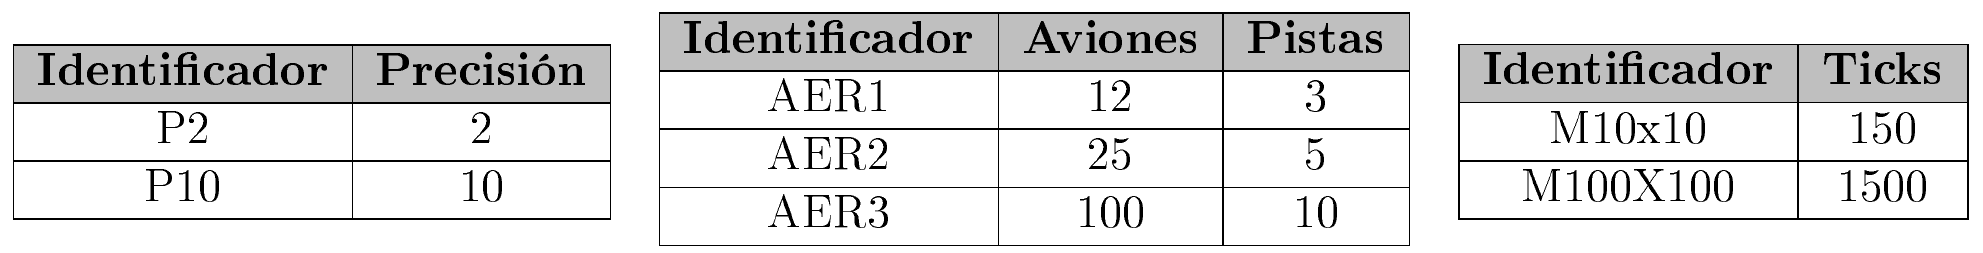
\includegraphics[width=1\textwidth]{images/chapter_4/tab_pev_variables}		
	\caption{Variables de cada individuo utilizadas en los experimentos}
	\label{tab:pev_variables}
\end{table}		

%\subsubsection{Algoritmos sin mejoras}

Primero, veamos cómo afecta a cada individuo modificar las variables de cada problema. La Figura \ref{fig:pev_secuencial} muestra dichos tiempos. La primera gráfica pertenece a los individuos binarios, y se puede apreciar que modificar la precisión no supone un coste elevado. Aumentar por cinco la precisión de la representación binaria (\textit{precisión(P10)/precisión(P2) = 5})) supone un aumento en el tamaño del array de bits de \textit{3.45} veces (\textit{76/22 = 3.45}) su tamaño. Sin embargo, el tiempo de ejecución no es proporcional al aumento del tamaño de bits, sino que es aproximadamente dos veces más lento. La gráfica del medio, representando a los individuos reales, tiene una mayor complejidad, por eso se puede apreciar una diferencia significativa al utilizar la segunda especificación (\textit{AER2}) con respecto a la tercera (\textit{AER3}), siendo seis veces más lenta. La última gráfica, muestra los resultados del problema de los individuos representados como árboles. Se puede observar que la primera función (línea azul) es cuatro veces más rápida que la segunda (línea roja). El tiempo de ejecución no es proporcional al número de \textit{ticks} ejecutados, pues el segundo problema ejecuta diez veces más \textit{ticks} que el primero. Las gráficas se muestran de forma lineal porque el número de generaciones es estático, es decir, solo aumenta el tamaño de la población. De otro modo sería exponencial y el tiempo de ejecución se elevaría.




\begin{figure}[h!]
	\hspace{-0.06\textwidth}
	\begin{tikzpicture}
		\begin{groupplot}[
			group style={
				group size=3 by 1,
				horizontal sep=0.78cm,
				vertical sep=0.5cm},
			width=0.40\textwidth,
			height=0.40\textwidth,
			tick label style={font=\tiny},
			title style={at={(0.05,0.925)},anchor=north west}
			]
			
			% 1
			\nextgroupplot[
			title={Binario},
			ylabel= Tiempo de ejecución (s),
			legend style={at={(0.5,1.05)},anchor=south,legend columns=-1},
			xtick={25, 500, 1000, 1500, 2000} 
			]
			\addplot [mark=none, color=blue] table [x index=0, y index=1, col sep=space] {files/pev.txt};
			\addplot [mark=none, color=red] table [x index=0, y index=2, col sep=space] {files/pev.txt};
			\addlegendentry{\tiny P2}
			\addlegendentry{\tiny P10}
			
			% 2
			\nextgroupplot[
			title={Real},
			xlabel=Tam. Población,
			legend style={at={(0.5,1.05)},anchor=south,legend columns=-1},
			xtick={25, 500, 1000, 1500, 2000} 
			]
			\addplot [mark=none, color=blue] table [x index=0, y index=3, col sep=space] {files/pev.txt};
			\addplot [mark=none, color=green] table [x index=0, y index=4, col sep=space] {files/pev.txt};
			\addplot [mark=none, color=red] table [x index=0, y index=5, col sep=space] {files/pev.txt};
			\addlegendentry{\tiny AER 1}
			\addlegendentry{\tiny AER 2}
			\addlegendentry{\tiny AER 3}
			
			% 3
			\nextgroupplot[
			title={Árbol},
			legend style={at={(0.5,1.05)},anchor=south,legend columns=-1},
			xtick={25, 500, 1000, 1500, 2000}
			]
			\addplot [mark=none, color=blue] table [x index=0, y index=6, col sep=space] {files/pev.txt};
			\addplot [mark=none, color=red] table [x index=0, y index=7, col sep=space] {files/pev.txt};
			\addlegendentry{\tiny M10X10}
			\addlegendentry{\tiny M100X100}
			
			
		\end{groupplot}        
	\end{tikzpicture}
	\caption{Tiempos de ejecución de los algoritmos evolutivos secuenciales}
	\label{fig:pev_secuencial}
\end{figure}





Antes de realizar las pruebas de las tres estrategias comentadas en la Sección \ref{cap:3_4}, vamos a comentar los tiempos de ejecución de las partes del algoritmo evolutivo, inicialización, evaluación, selección, cruce y mutación. Cada prueba mide el tiempo de ejecución para un individuo (dos individuos en el caso del cruce). La Tabla \ref{tab:pev}, muestra los resultados obtenidos, resaltando en rojo aquellos métodos que más tiempo consumen. Los resultados de los individuos binarios muestran que el cruce y la mutación son las partes que más tiempo consumen (inicialización no cuenta, pues solo se ejecuta una vez). La evaluación de estos individuos recorre los bits para convertirlo a un número real, pero no cambian los valores, reduciendo así el tiempo de ejecución. Los individuos reales y árboles tienen una función de evaluación con mayor complejidad, lo que provoca que esta parte sea la que más tarde. 



\begin{table}[!h]
	\centering
	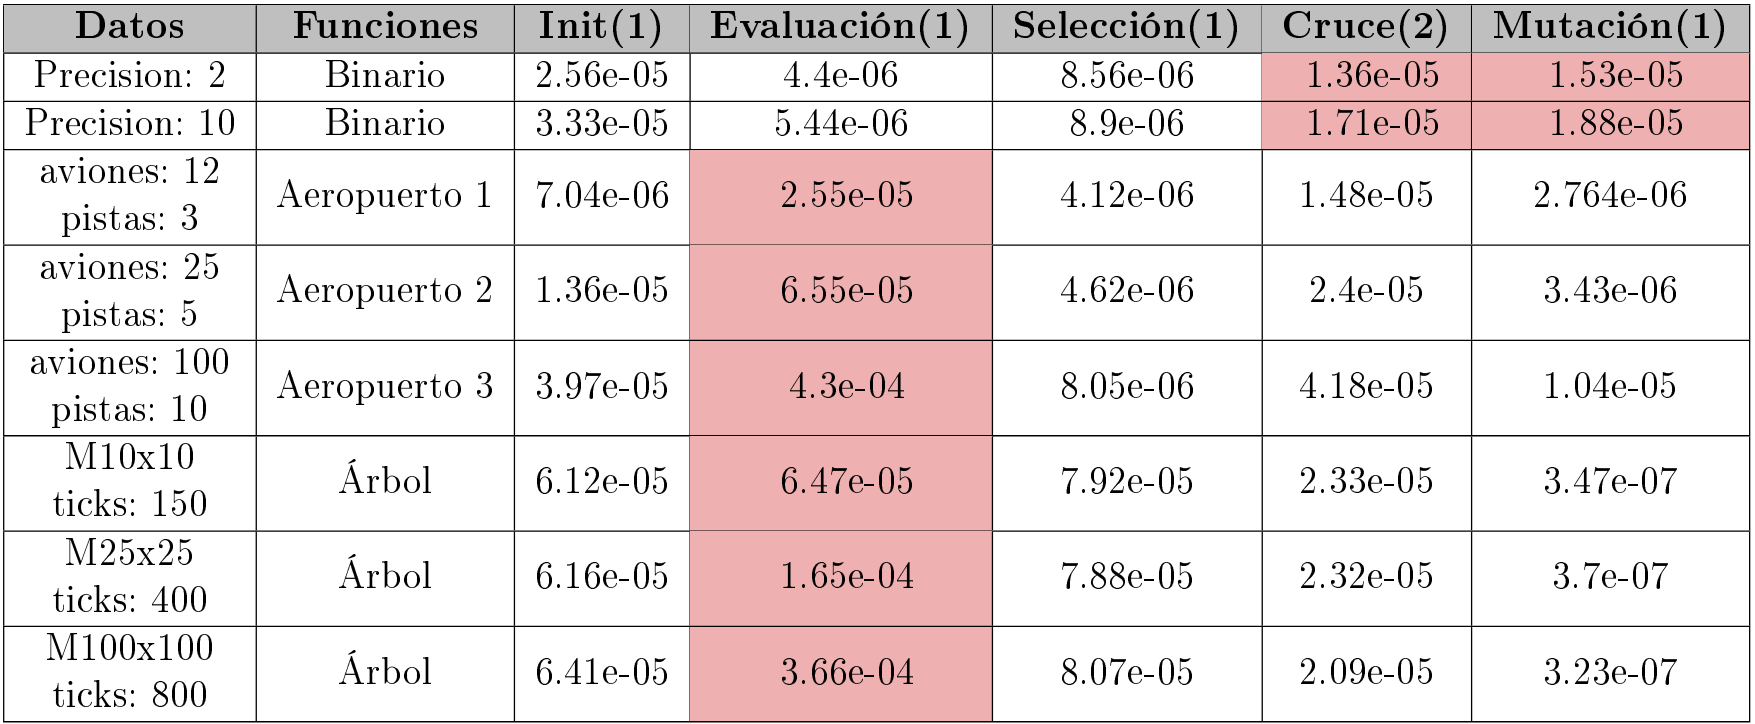
\includegraphics[width=1\textwidth]{images/chapter_4/tabla_pev}		
	\caption{Tiempos unitarios de las partes del algoritmo evolutivo para cada individuo}
	\label{tab:pev}
\end{table}

\begin{comment}[!h]
	\centering
	\begin{tabular}{|c|c|c|c|c|c|c|}
		\hline
		\rowcolor{lightgray}
		\textbf{Datos} & \textbf{Funciones} & \textbf{Init(1)} & \textbf{Evaluación(1)} & \textbf{Selección(1)} & \textbf{Cruce(2)} & \textbf{Mutación(1)} \\
		\hline
		Precision: 2 & Binario & 2.56e-05 & 4.4e-06 & 8.56e-06 & \cellcolor{redcell} 1.36e-05 & \cellcolor{redcell} 1.53e-05 \\
		\hline
		Precision: 10 & Binario & 3.33e-05 & 5.44e-06 & 8.9e-06 & \cellcolor{redcell} 1.71e-05 & \cellcolor{redcell} 1.88e-05 \\
		\hline
		\makecell{aviones: 12 \\ pistas: 3} & Aeropuerto 1 & 7.04e-06 & \cellcolor{redcell} 2.55e-05 & 4.12e-06 & 1.48e-05 & 2.764e-06 \\
		\hline
		\makecell{aviones: 25 \\ pistas: 5} & Aeropuerto 2 & 1.36e-05 & \cellcolor{redcell} 6.55e-05 & 4.62e-06 & 2.4e-05 & 3.43e-06 \\
		\hline
		\makecell{aviones: 100 \\ pistas: 10} & Aeropuerto 3 & 3.97e-05 & \cellcolor{redcell} 4.3e-04 & 8.05e-06 & 4.18e-05 & 1.04e-05 \\
		\hline
		\makecell{M10x10 \\ ticks: 150} & Árbol & 6.12e-05 & \cellcolor{redcell} 6.47e-05 & 7.92e-05 & 2.33e-05 & 3.47e-07 \\
		\hline
		\makecell{M25x25 \\ ticks: 400} & Árbol & 6.16e-05 & \cellcolor{redcell} 1.65e-04 & 7.88e-05 & 2.32e-05 & 3.7e-07 \\
		\hline
		\makecell{M100x100 \\ ticks: 800} & Árbol & 6.41e-05 & \cellcolor{redcell} 3.66e-04 & 8.07e-05 & 2.09e-05 & 3.23e-07 \\
		\hline
	\end{tabular}
	\caption{PEV - Tiempos de cada método}
	\label{tab:adujsfh}
\end{comment}




Cabe destacar que estos tiempos no son la única medida que se necesita para las estrategias. El tiempo de comunicación entre procesos va a aumentar considerablemente el tiempo de ejecución, siendo, el individuo binario, el tipo de individuo que más desventaja tiene, pues al tener más datos consumirá más tiempo al enviar y recibir mensajes.





%\subsubsection{Mejora 2: Modelo de islas}
Empezando con las estrategias de la Sección \ref{cap:3_4}, \textit{modelo de islas} consiste en dividir los individuos de la población entre ``islas'' (procesos). La configuración de las islas no influye en la reducción del tiempo de ejecución, en una configuración u otra solo varía como se garantiza la supervivencia de los mejores individuos en la población general. Si usamos la topología en estrella, hay que reservar un proceso para que actúe como \textit{master} para que éste realice el proceso de comunicación cada \textit{X} generaciones. Las demás topologías (red y anillo) no tienen un proceso \textit{master} por lo que se optimiza de mejor forma los recursos computacionales. Las pruebas realizadas a continuación se han ejecutado con la topología de anillo, con cuatro procesos. La Figura \ref{fig:pev_mpi2} muestra los resultados en forma de malla de \textit{2x2} con los tiempos de ejecución de los algoritmos evolutivos con esta estrategia, separando las pruebas de los individuos reales (segunda fila) debido a la diferencia de tiempos con respecto al problema con mayor tamaño (\textit{AER3}). Como se puede apreciar, se logra obtener una reducción del tiempo de ejecución proporcional al número de procesos ejecutados. El estudio de los \textit{speed-ups} (figura \ref{fig:pev_mpi1_speedups}) para los problemas de mayor tamaño de cada individuo, confirma la proporcionalidad de la reducción del tiempo de ejecución con respecto al número de procesos ejecutados. La primera gráfica de la primera fila (ver Figura \ref{fig:pev_mpi2}) muestra los resultados obtenidos para los individuos binarios, consiguiendo reducir el tiempo de ejecución. La segunda gráfica de esta misma fila muestra los resultados para los árboles, cuyo tiempo de ejecución de la estrategia sobre el segundo problema (\textit{1500 ticks}) es aproximadamente igual a los obtenidos para la ejecución secuencial del primer problema (\textit{150 ticks}). Como se usan cuatro procesos y el primer problema es cuatro veces más rápido que el segundo, los resultados de estas ejecuciones se solapan, provocando que la línea verde y azul coincidan. Las gráficas de los individuos reales de la segunda fila, muestran un mismo comportamiento que las gráficas anteriores con respecto a la reducción del tiempo de ejecución.




\begin{figure}[h!]
	\centering
	\hspace{-0.06\textwidth}
	\begin{tikzpicture}
		\begin{groupplot}[group style={
				group size=2 by 2,
				horizontal sep=1.2cm, 
				vertical sep=1.75cm},  
			width=0.47\textwidth, height=0.30\textheight, 	
			tick label style={font=\tiny},
			title style={at={(0.05,0.915)},anchor=north west} 	
			]
			
			% 1
			\nextgroupplot[title=Binario, 
			legend style={at={(0.5,1.05)},anchor=south,legend columns=2},
			xtick={25, 500, 1000, 1500, 2000}]
			\addplot [mark=none, color=blue] table [x index=0, y index=1, col sep=space] {files/pev_2mpi.txt};
			\addplot [mark=none, color=red] table [x index=0, y index=2, col sep=space] {files/pev_2mpi.txt};
			\addplot [mark=none, color=black] table [x index=0, y index=3, col sep=space] {files/pev_2mpi.txt};
			\addplot [mark=none, color=darkgreen] table [x index=0, y index=4, col sep=space] {files/pev_2mpi.txt};
			\addlegendentry{\tiny P2}
			\addlegendentry{\tiny P10}
			\addlegendentry{\tiny P2\_MPI(4)}
			\addlegendentry{\tiny P10\_MPI(4)}
			
			% 2
			\nextgroupplot[title=Árbol,
			legend style={at={(0.5,1.05)},anchor=south,legend columns=2},
			xtick={25, 500, 1000, 1500, 2000},
			xlabel near ticks]  
			\addplot [mark=none, color=blue] table [x index=0, y index=11, col sep=space] {files/pev_2mpi.txt};
			\addplot [mark=none, color=red] table [x index=0, y index=12, col sep=space] {files/pev_2mpi.txt};
			\addplot [mark=none, color=black] table [x index=0, y index=13, col sep=space] {files/pev_2mpi.txt};  
			\addplot [mark=none, color=darkgreen] table [x index=0, y index=14, col sep=space] {files/pev_2mpi.txt};  
			\addlegendentry{\tiny M10X10}
			\addlegendentry{\tiny M100X100}
			\addlegendentry{\tiny M10X10\_MPI(4)}
			\addlegendentry{\tiny M100X100\_MPI(4)}
			
			
			% 3
			\nextgroupplot[title=Real, 
			legend style={at={(0.5,1.05)},anchor=south,legend columns=2},
			xtick={25, 500, 1000, 1500, 2000}]
			\addplot [mark=none, color=blue] table [x index=0, y index=5, col sep=space] {files/pev_2mpi.txt};			
			\addplot [mark=none, color=red] table [x index=0, y index=7, col sep=space] {files/pev_2mpi.txt};
			\addplot [mark=none, color=black] table [x index=0, y index=6, col sep=space] {files/pev_2mpi.txt};
			\addplot [mark=none, color=darkgreen] table [x index=0, y index=8, col sep=space] {files/pev_2mpi.txt};
			\addlegendentry{\tiny AER 1}
			\addlegendentry{\tiny AER 2}
			\addlegendentry{\tiny AER 1\_MPI(4)}
			\addlegendentry{\tiny AER 2\_MPI(4)}
			
			%4
			\nextgroupplot[title=Real,
			legend style={at={(0.5,1.05)},anchor=south,legend columns=-1},
			xtick={25, 500, 1000, 1500, 2000},
			xlabel near ticks] 
			\addplot [mark=none, color=red] table [x index=0, y index=9, col sep=space] {files/pev_2mpi.txt};
			\addplot [mark=none, color=black] table [x index=0, y index=10, col sep=space] {files/pev_2mpi.txt};
			\addlegendentry{\tiny AER 3}
			\addlegendentry{\tiny AER 3\_MPI(4)}
			
			
			
		\end{groupplot}
		
		% Eje X
		\node at ($(group c2r2.south east)!0.5!(group c1r2.south west)$) [below=0.7cm] {Tam. Población};
		
		% Eje Y
		\node at ($(group c1r2.south west)!0.75!(group c1r1.north west)$) [left=0.85cm,rotate=90] {\footnotesize Tiempo de ejecución (s)};
		
	\end{tikzpicture}
	\caption{Tiempos de ejecución de la estrategia \textit{modelo de islas} de los algoritmos evolutivos en ordenador de propósito general}
	\label{fig:pev_mpi2}
\end{figure}


\begin{figure}[!h]
	\centering
	\begin{tikzpicture}
		\begin{axis}[
			xlabel={Tam. Población},
			ylabel={speed-up},
			legend pos=south east,
			grid=major,
			width=0.55\textwidth,
			height=0.40\textwidth,
			scaled x ticks=false,
			ymin=0, 
			ymax=5
			]
			
			
			\addplot [mark=diamond*, color=darkgreen, line width=1.2pt] table [x index=0, y index=1, col sep=space] {files/pev_2mpi_speedup.txt};
			\addplot [mark=none, color=blue, line width=0.8pt] table [x index=0, y index=2, col sep=space] {files/pev_2mpi_speedup.txt};
			\addplot [mark=none, color=red, line width=0.8pt] table [x index=0, y index=3, col sep=space] {files/pev_2mpi_speedup.txt};
			\addplot [mark=none, color=black, line width=0.8pt] table [x index=0, y index=4, col sep=space] {files/pev_2mpi_speedup.txt};
			
			
			\addlegendentry{Ideal}
			\addlegendentry{P10}
			\addlegendentry{AER3}
			\addlegendentry{M100X100}
			
			
		\end{axis}
	\end{tikzpicture}
	\caption{\textit{Speed-ups} de la estrategia \textit{modelo de islas} de los algoritmos evolutivos en ordenador de propósito general}
	\label{fig:pev_mpi1_speedups}
\end{figure}


\newpage



%\subsubsection{Mejora 1: Dividir con el master}
La estrategia de \textit{dividir la población} entre los procesos tiene una complejidad mayor en lo que a lógica de programación se trata. Con el modelo de comunicación \textit{Master-Worker} y una población de individuos, el \textit{master} se encarga de dividir y enviar a los \textit{workers} la población sobre la cual tienen que ejecutar las partes del algoritmo: cruce, mutación y evaluación en cada generación. Las siguientes pruebas se ejecutan con cuatro \textit{workers}, cinco procesos en total contando al \textit{master}. La Figura \ref{fig:pev_mpi1_1} muestra, en forma de malla \textit{2x2}, los resultados obtenidos para los tres diferentes individuos. 

La primera gráfica de la primera fila muestra los resultados de los individuos binarios, unos tiempos de ejecución muy parecidos. Para el primer problema, usando \textit{22} bits, no se logra reducir el tiempo de ejecución, pues se puede ver que empiezan de forma similar, pero con mil individuos se empiezan a distanciar. Esto no ocurre con el segundo problema (\textit{77} bits por individuo), la estrategia logra reducir levemente el tiempo de ejecución, y con dos mil individuos, la ejecución sigue siendo un poco más rápida. El factor que frena a esta estrategia de reducir el tiempo de ejecución es la complejidad de las operaciones a realizar en cada parte del algoritmo, pues son muy simples. Además, la comunicación entre procesos al enviar y recibir muchos bits aumenta el tiempo de ejecución. La segunda gráfica de la misma fila (ver Figura \ref{fig:pev_mpi1_1}) muestra los resultados de los individuos representados como árboles, siendo resultados parecidos a la anterior gráfica comentada. Para el primer problema (\textit{150 ticks}) no se consigue reducir el tiempo de ejecución, no obstante, para el segundo si se logra, obteniendo, para la última población (\textit{2000} individuos), un \textit{speed-up} de \textit{1.84}. Las pruebas en los individuos reales, al igual que para la estrategia anterior, se dividen en dos gráficas para poder ver con mayor exactitud los resultados obtenidos, estas gráficas se sitúan en la segunda fila (ver Figura \ref{fig:pev_mpi1_1}). Al contrario que los otros dos individuos, este individuo si alcanza una reducción del tiempo de ejecución con todos los tamaños de problemas. La gráfica de la izquierda muestra que la estrategia en los dos primeros tamaños alcanza un buen rendimiento, pero el tercer problema, al ser más grande, tiene una reducción del tiempo de ejecución más notoria. Como muestra la gráfica de la derecha, se puede alcanzar un \textit{speed-up} de \textit{2.81}.

\begin{figure}[!h]
	\centering
	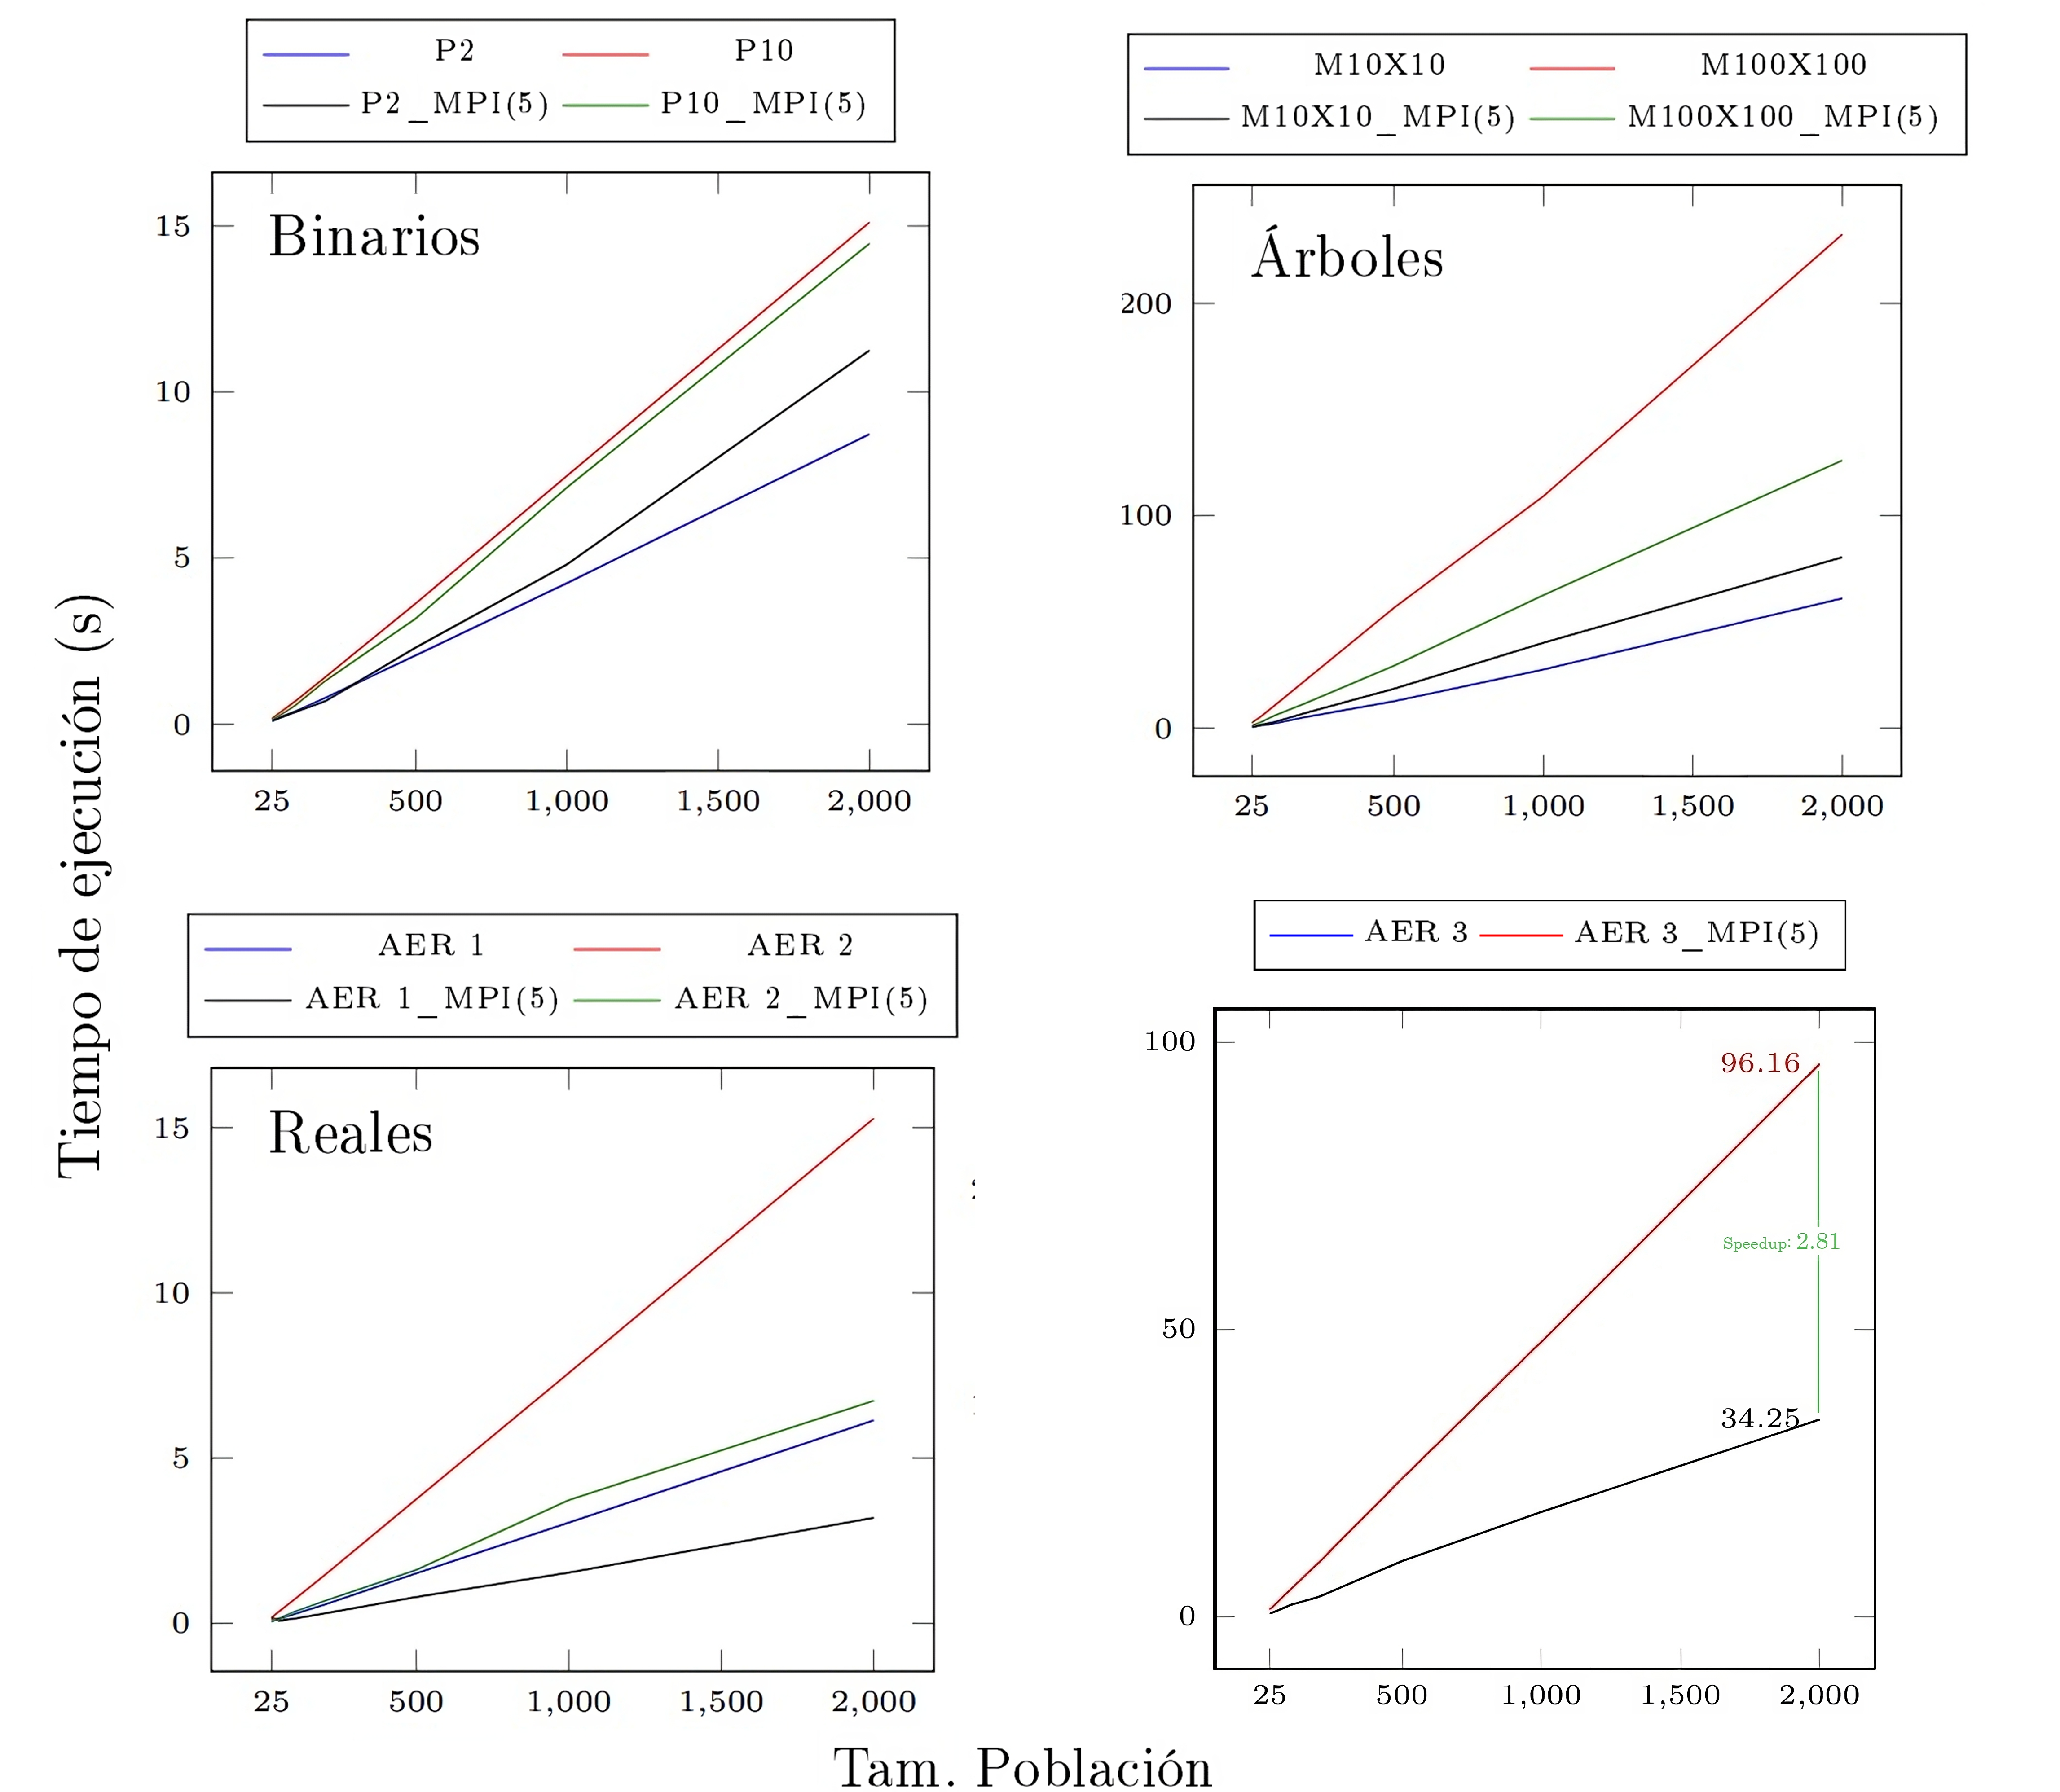
\includegraphics[width=0.80\textwidth]{images/chapter_4/pev_1_1mpi}
	\caption{Tiempo de ejecución de la estrategia \textit{dividir población} de los algoritmos evolutivos de en ordenador de propósito general}
	\label{fig:pev_mpi1_1}			
\end{figure}
\newpage

\begin{comment}[!h]
	\hspace{-0.06\textwidth}
	\begin{tikzpicture}
		\begin{groupplot}[group style={
				group size=3 by 1,
				horizontal sep=0.78cm, 
				vertical sep=0.5cm}, 
			width=0.40\textwidth, height=0.35\textwidth, 
			tick label style={font=\tiny},
			title style={at={(0.05,0.915)},anchor=north west} 	
			]
			
			% 1
			\nextgroupplot[title={Binarios}, ylabel=Tiempo de ejecución (s),
			legend style={at={(0.5,1.05)},anchor=south,legend columns=2},
			xtick={25, 500, 1000, 1500, 2000}]
			\addplot [mark=none, color=blue] table [x index=0, y index=1, col sep=space] {files/pev_1_1mpi.txt};
			\addplot [mark=none, color=red] table [x index=0, y index=2, col sep=space] {files/pev_1_1mpi.txt};
			\addplot [mark=none, color=black] table [x index=0, y index=3, col sep=space] {files/pev_1_1mpi.txt};
			\addplot [mark=none, color=darkgreen] table [x index=0, y index=4, col sep=space] {files/pev_1_1mpi.txt};
			\addlegendentry{\tiny P2}
			\addlegendentry{\tiny P10}
			\addlegendentry{\tiny P2\_MPI(5)}
			\addlegendentry{\tiny P10\_MPI(5)}
			
			% 2
			\nextgroupplot[title={Reales}, xlabel=Tam. Población,
			legend style={at={(0.5,1.05)},anchor=south,legend columns=2},
			xtick={25, 500, 1000, 1500, 2000}]
			\addplot [mark=none, color=blue] table [x index=0, y index=5, col sep=space] {files/pev_1_1mpi.txt};	
			\addplot [mark=none, color=red] table [x index=0, y index=7, col sep=space] {files/pev_1_1mpi.txt};
			\addplot [mark=none, color=black] table [x index=0, y index=6, col sep=space] {files/pev_1_1mpi.txt};
			\addplot [mark=none, color=darkgreen] table [x index=0, y index=8, col sep=space] {files/pev_1_1mpi.txt};
			\addlegendentry{\tiny AER 1}
			\addlegendentry{\tiny AER 2}
			\addlegendentry{\tiny AER 1\_MPI(5)}
			\addlegendentry{\tiny AER 2\_MPI(5)}
			
			
			% 3
			\nextgroupplot[title={Árboles},
			legend style={at={(0.5,1.05)},anchor=south,legend columns=2},
			xtick={25, 500, 1000, 1500, 2000}]
			\addplot [mark=none, color=blue] table [x index=0, y index=9, col sep=space] {files/pev_1_1mpi.txt};			
			\addplot [mark=none, color=red] table [x index=0, y index=10, col sep=space] {files/pev_1_1mpi.txt};		
			\addplot [mark=none, color=black] table [x index=0, y index=11, col sep=space] {files/pev_1_1mpi.txt};
			\addplot [mark=none, color=darkgreen] table [x index=0, y index=12, col sep=space] {files/pev_1_1mpi.txt};	
			\addlegendentry{\tiny M10X10}
			\addlegendentry{\tiny M100X100}
			\addlegendentry{\tiny M10X10\_MPI(5)}
			\addlegendentry{\tiny M100X100\_MPI(5)}
			
		\end{groupplot}	
		
		
		%\node at ($(group c1r1.south)!0.5!(group c2r1.south) + (0,-0.4cm)$) [below] {Num. Generaciones};
		
	\end{tikzpicture}
	\caption{Tiempos de ejecución de la estrategia dividir población de los algoritmos evolutivos en ordenador de propósito general}
	\label{fig:pev_mpi1_1AUX}
\end{comment}

\begin{comment}[!h]
	\centering
	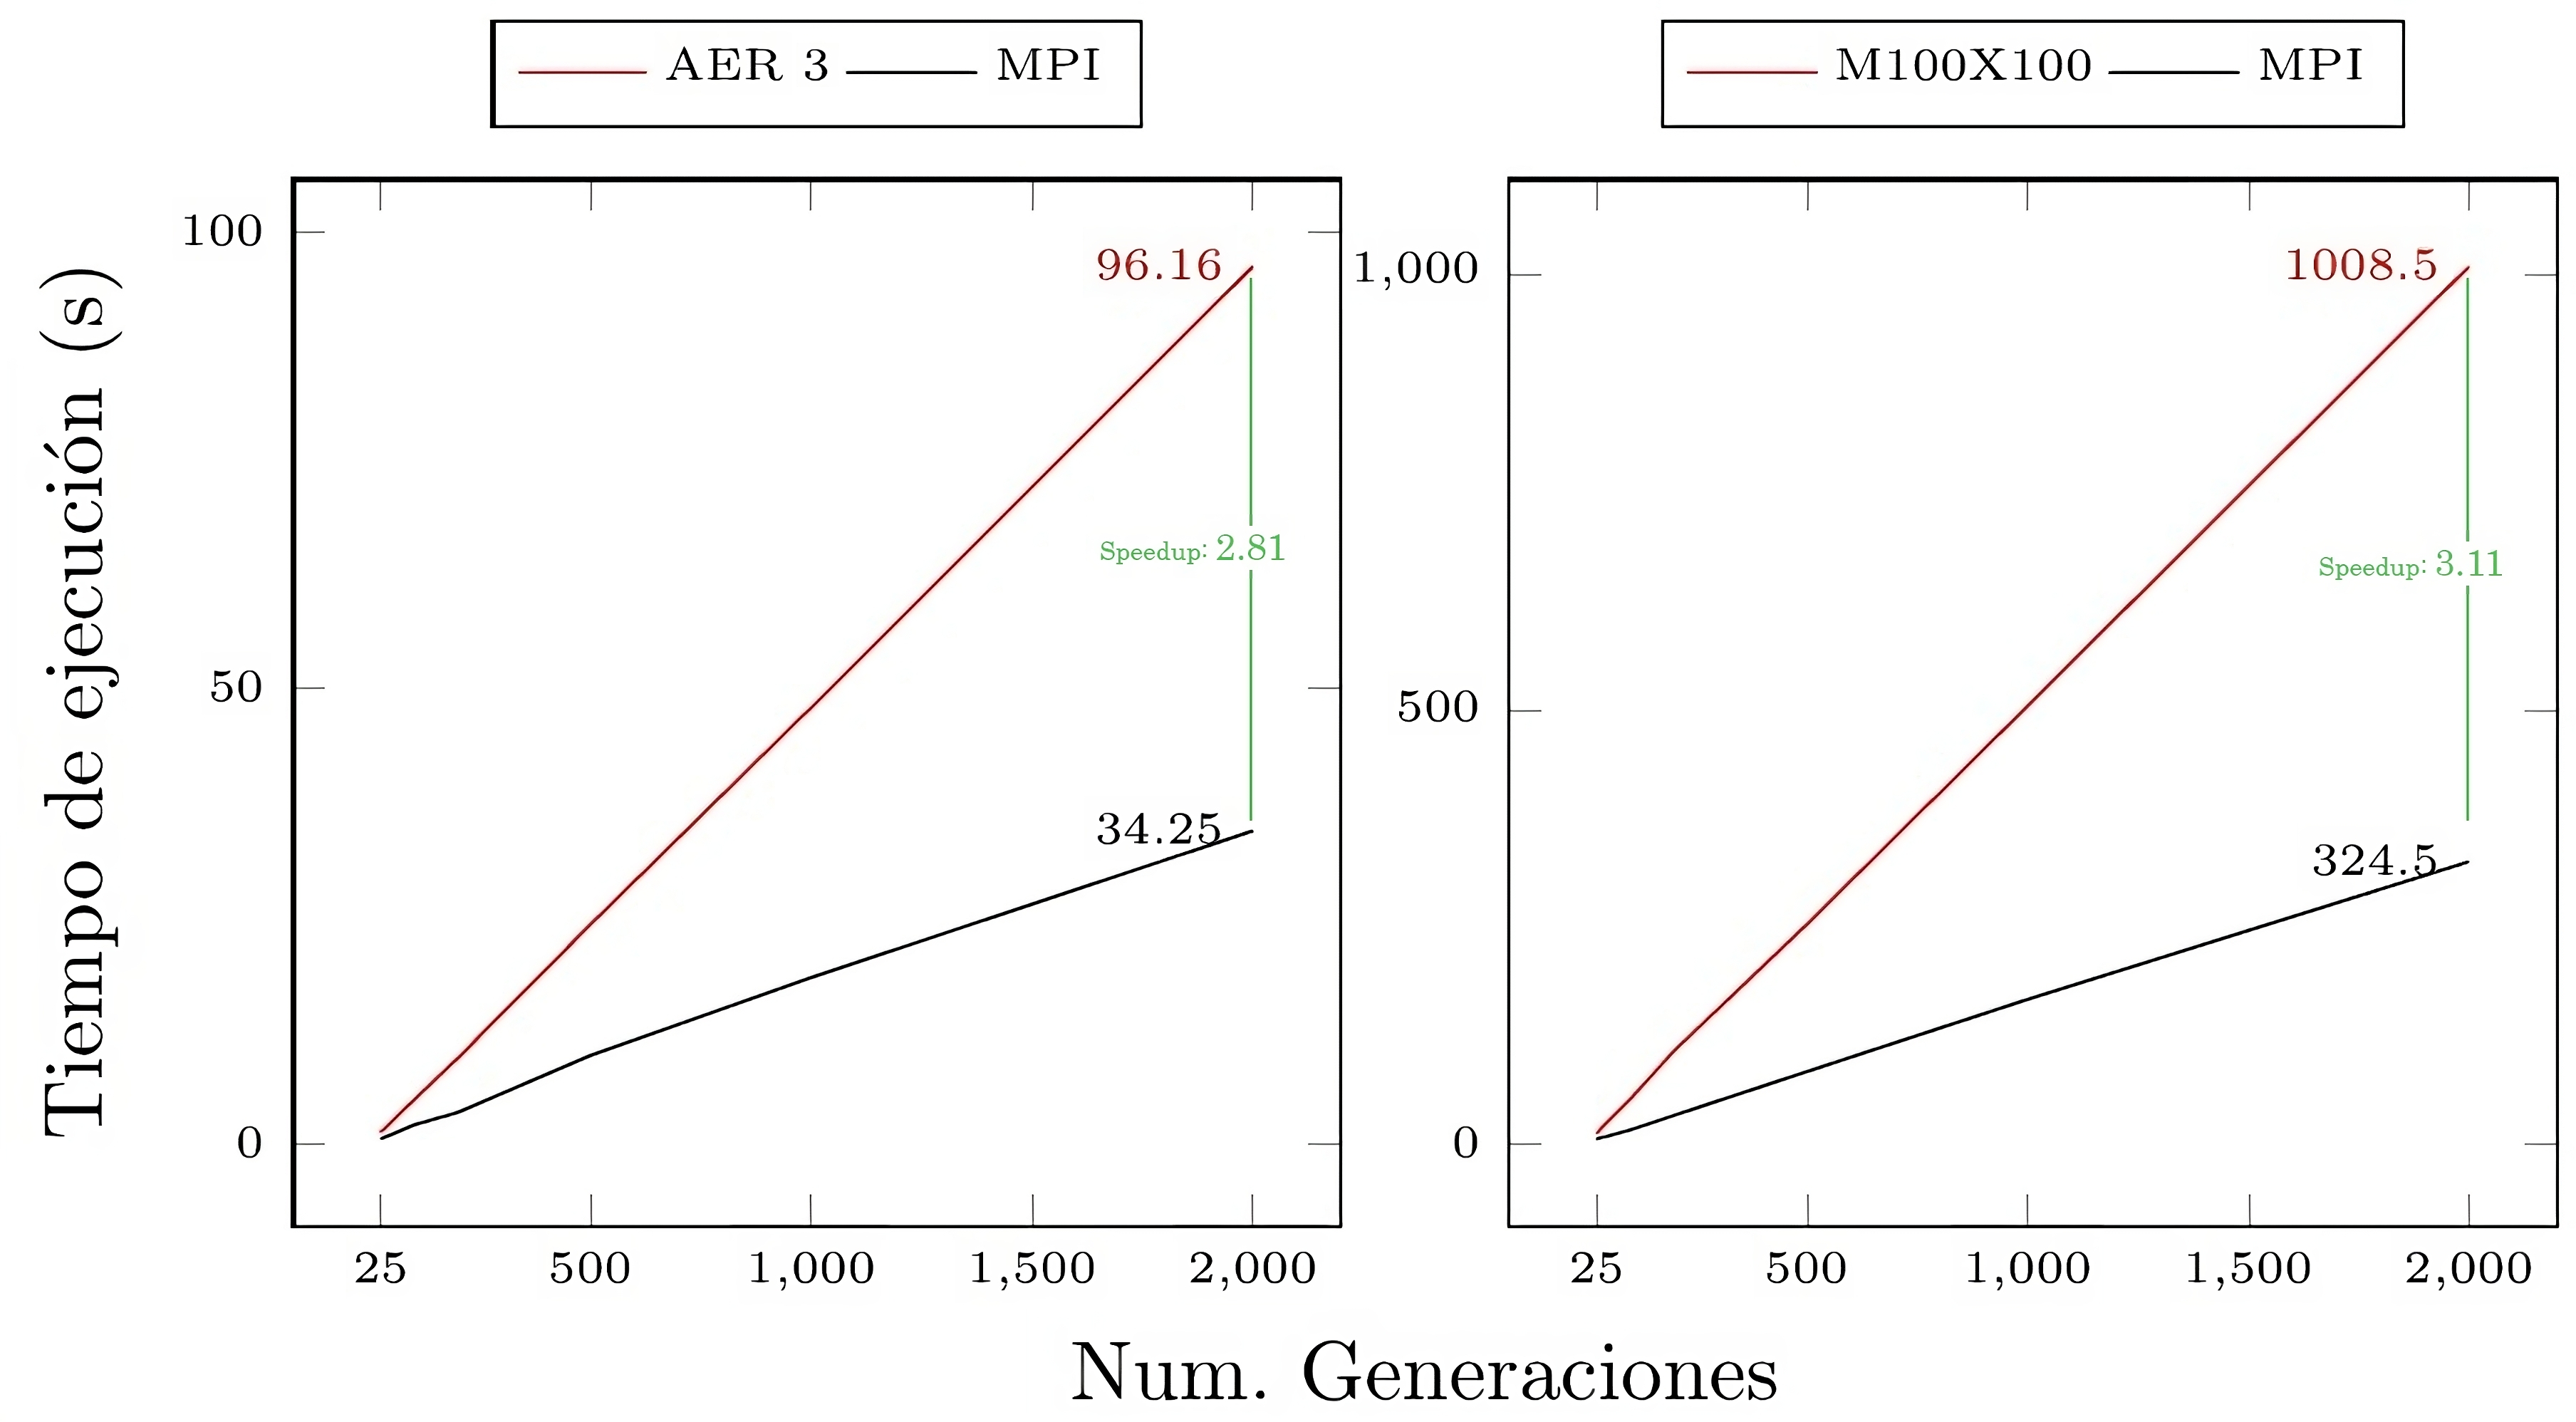
\includegraphics[width=0.45\textwidth]{images/chapter_4/pev_mpi1}
	\caption{Tiempo de ejecución de la estrategia dividir población para problemas de mayor tamaño de individuos reales de los algoritmos evolutivos de en ordenador de propósito general}
	\label{fig:pev_mpi1_2AUX}			
\end{comment}



%\subsubsection{Mejora 3: PipeLine}

La estrategia \textit{pipeline} mezcla el modelo \textit{Master-Worker} con segmentación. El proceso \textit{master} se encarga de generar una población dividida entre \textit{N} (número de \textit{workers}) subpoblaciones que envía al siguiente proceso (primer \textit{worker}). Cuando genera todas las subpoblaciones, se queda en un estado de recepción de mejores individuos. Cada proceso envía a su siguiente los datos procesados según su tarea, generando un flujo constante de trabajo. Esta estrategia varía para cada individuo, debido a que los tiempos en cada parte del algoritmo son distintos para cada uno. Estos tiempos se estudiaron previamente en la Tabla \ref{tab:pev}. La primera prueba se realiza sobre los individuos binarios, con \textit{\textit{precision=10}}, cuyos procesos ejecutados se estructuran de la siguiente forma:

\begin{itemize}
	\item Con cuatro procesos el \textit{master} se encarga de inicializar. Los \textit{workers} se dividen en tres pipes; el primer pipe se encarga de la evaluación y selección, el segundo del cruce y el tercero de la mutación.
	\item Con siete procesos: se duplica la ayuda para los \textit{workers} en cada pipe. 
\end{itemize}


Los resultados son plasmados en la Figura \ref{pev:estrategia_mpi3_1}, logrando reducir satisfactoriamente el tiempo de ejecución. El funcionamiento de \textit{pipeline} reduce el tiempo de paso de mensajes, al optimizar la paralelización de las partes del algoritmo. 

\begin{figure}[!h]
	\centering
	\begin{tikzpicture}
		\begin{axis}[
			xlabel={Tam. Poblacion},
			ylabel={Tiempo de ejecución (s)},
			xtick={25,200,500,1000,1500,2000},
			legend pos=north west,
			grid=major,
			width=0.70\textwidth,
			height=0.35\textwidth
			]				
			
			xtick={25, 500, 1000, 1500, 2000}]
			\addplot [mark=none, color=red] table [x index=0, y index=1, col sep=space] {files/pev_3mpi.txt};
			\addplot [mark=none, color=darkgreen] table [x index=0, y index=2, col sep=space] {files/pev_3mpi.txt};
			\addplot [mark=none, color=blue] table [x index=0, y index=3, col sep=space] {files/pev_3mpi.txt};
			
			\addlegendentry{\tiny P10}
			\addlegendentry{\tiny MPI(4)}
			\addlegendentry{\tiny MPI(7)}
			
		\end{axis}
	\end{tikzpicture}
	\caption{Tiempo de ejecución de la estrategia \textit{pipeline} en los individuos binarios del algoritmo evolutivo en ordenador de propósito general}
	\label{pev:estrategia_mpi3_1}
\end{figure}

Los individuos reales y árboles tienen tiempos de ejecución muy parecidos. Es por eso que se obtendrían los mismos resultados al aplicar la misma repartición de tareas, siendo esta la siguiente:		
\begin{itemize}
	\item Con seis procesos: el \textit{master} se encarga de inicializar. Los \textit{workers} con \textit{ids} en el intervalo \textit{[1-4]} se encargan de la evaluación, pues esta parte del algoritmo consume cuatro veces más tiempo que los restantes. El último worker se encarga de la selección, cruce y mutación.
	\item Con diez procesos: se duplica la ayuda para los \textit{workers} en la función de evaluación. Alcanzando, con este reparto de tareas, una igualdad en los tiempos de ejecución de los dos tipos de procesos \textit{worker}. Es decir, con ocho \textit{workers} se logra reducir el tiempo de ejecución al mismo tiempo que el del \textit{worker} que realiza las otras partes del algoritmo.
\end{itemize}

Como muestra la Figura \ref{fig:estrategia_mpi3_2}, los individuos reales también presentan un buen rendimiento. Aunque duplicando los procesos \textit{workers} de la función de evaluación (linea azul), se obtiene unos tiempos de ejecución similares a los obtenidos con seis procesos.


\begin{figure}[!h]
	\centering
	\begin{tikzpicture}
		\begin{axis}[
			xlabel={Tam. Poblacion},
			ylabel={Tiempo de ejecución (s)},
			xtick={25,200,500,1000,1500,2000},
			legend pos=north west,
			grid=major,
			width=0.70\textwidth,
			height=0.35\textwidth
			]				
			
			xtick={25, 500, 1000, 1500, 2000}]
			\addplot [mark=none, color=red] table [x index=0, y index=4, col sep=space] {files/pev_3mpi.txt};			
			\addplot [mark=none, color=darkgreen] table [x index=0, y index=5, col sep=space] {files/pev_3mpi.txt};
			\addplot [mark=none, color=blue] table [x index=0, y index=6, col sep=space] {files/pev_3mpi.txt};	
			\addlegendentry{\tiny AER3}
			\addlegendentry{\tiny MPI(6)}
			\addlegendentry{\tiny MPI(10)}
			
		\end{axis}
	\end{tikzpicture}
	\caption{Tiempo de ejecución de la estrategia pipeline en los individuos reales del algoritmo evolutivo en ordenador de propósito general}
	\label{fig:estrategia_mpi3_2}
\end{figure}



\begin{comment}[h!]
	\centering
	\begin{tikzpicture}
		\begin{groupplot}[group style={
				group size=3 by 1,
				horizontal sep=0.78cm, 
				vertical sep=0.5cm},
			width=0.40\textwidth, height=0.40\textwidth, 
			tick label style={font=\tiny} 
			]
			
			% 1
			\nextgroupplot[title={}, ylabel=Tiempo de ejecución (s),
			legend pos=north west,
			xtick={25, 500, 1000, 1500, 2000}]
			\addplot [mark=none, color=red] table [x index=0, y index=1, col sep=space] {files/pev_3mpi.txt};
			\addplot [mark=none, color=darkgreen] table [x index=0, y index=2, col sep=space] {files/pev_3mpi.txt};
			\addplot [mark=none, color=blue] table [x index=0, y index=3, col sep=space] {files/pev_3mpi.txt};							
			\addlegendentry{\tiny P10}
			\addlegendentry{\tiny MPI(4)}
			\addlegendentry{\tiny MPI(7)}
			
			
			% 2
			\nextgroupplot[title={},
			legend pos=north west,
			xtick={25, 500, 1000, 1500, 2000}]
			\addplot [mark=none, color=red] table [x index=0, y index=4, col sep=space] {files/pev_3mpi.txt};			
			\addplot [mark=none, color=darkgreen] table [x index=0, y index=5, col sep=space] {files/pev_3mpi.txt};
			\addplot [mark=none, color=blue] table [x index=0, y index=6, col sep=space] {files/pev_3mpi.txt};	
			\addlegendentry{\tiny AER3}
			\addlegendentry{\tiny MPI(6)}
			\addlegendentry{\tiny MPI(10)}
			
		\end{groupplot}	
		
		\node at ($(group c1r1.south)!0.5!(group c2r1.south) + (0,-0.4cm)$) [below] {Num. Generaciones};
	\end{tikzpicture}
	\caption{MPI3 - PipeLine}
\end{comment}
\begin{comment}
	\begin{mdframed}[roundcorner=5pt]
		\normalsize
		\textbf{Binarios}	
		
		\small
		\color{darkgreen} 1. Cuatro procesos: \color{black}
		\vspace{-0.3cm}
		\scriptsize
		\begin{itemize}
			\item Master se encarga de inicializar
			\vspace{-0.1cm}
			\item Worker1: evaluación y selección, procesos que no tardan mucho en ejecutarse.
			\vspace{-0.1cm}
			\item Worker2: cruce
			\vspace{-0.1cm}
			\item Worker3: mutación
		\end{itemize}
		\small
		\color{blue} 2. Siete procesos. \color{black} 	\scriptsize	Se duplica el numero de workers en cada pipe.	
		
		\vspace{0.2cm}
		
		\normalsize		
		\textbf{Reales} \small (Solo aumenta el número de workers en el método de evaluación.)	
		
		
		\normalsize		
		\color{darkgreen} 1. Seis procesos: \color{black}
		\vspace{-0.3cm}
		\scriptsize
		\begin{itemize}			
			\item Master se encarga de inicializar
			\vspace{-0.1cm}
			\item Worker [1, 4]: evaluación, función que más tarda			
			\vspace{-0.1cm}
			\item Worker 5:  selección, cruce y mutación						
			\vspace{-0.1cm}
		\end{itemize}
		\small
		\color{blue} 2. Diez procesos. \color{black} \scriptsize Se duplica el numero de workers en cada pipe.
		
		\vspace{0.2cm}
		\normalsize
		\textbf{Arboles:} \small Es igual que la implementación de individuos reales, pues la evaluación es el método que más tarda.			
	\end{mdframed}
\end{comment}





%\subsubsection{Cluster}
En el \textit{cluster} se han realizado pruebas para las estrategias de \textit{dividir la población} y \textit{pipeline}. La estrategia de \textit{modelo de islas} no se ha realizado debido a que ya se han realizado varias pruebas en el sistema distribuido con esta estructura de dividir el algoritmo secuencial entre varios procesos. Ambas pruebas tienen los siguientes tamaños de poblaciones [\textit{1000}, \textit{2000}, \textit{5000}, \textit{7000}]. La estrategia de \textit{dividir la población} se ejecuta sobre individuos reales, con \textit{10}, \textit{20}, \textit{50}, y \textit{100} procesos. La Figura \ref{fig:pev_cluster1} muestra dichos resultados. Como se puede ver en el gráfico, a partir de \textit{20} procesos la reducción del tiempo de ejecución empieza a ralentizarse. En el último tamaño de poblaciones, se logra obtener un menor tiempo con \textit{50} procesos que al usar \textit{100}. La sobrecarga producida por la comunicación entre un número elevado de procesos \textit{workers} y el \textit{master} generan dichos resultados.

La estrategia de \textit{pipeline} se ejecuta sobre individuos árboles, siguiendo el mismo reparto de tareas que la utilizada para los individuos reales. Como se comentó antes, al llegar a \textit{10} procesos se alcanza una igualdad en los tiempos de ejecución. Es por esos que los procesos ejecutados para esta prueba son múltiplos de este número, siendo \textit{10}, \textit{20}, \textit{40} y \textit{80}. Entre cada prueba se duplican los procesos involucrados en cada tarea, incluyendo la inicialización de los individuos realizada por el proceso \textit{master}. Los resultados obtenidos son mostrados en la Figura \ref{fig:pev_cluster2}. Se puede apreciar un comportamiento similar a la Figura \ref{fig:pev_cluster1} del párrafo anterior, en el cual al llegar a \textit{40} procesos se obtienen aproximadamente los mismos resultados que duplicando los procesos.




\begin{figure}[!h]
	\hspace{-0.07\textwidth}
	\begin{tikzpicture}
		\begin{axis}[
			xlabel={Tam. Población ($10^3$)},
			ylabel={Tiempo de ejecución (s)},
			legend style={at={(1.02,0.5)}, anchor=west},
			grid=major,
			width=\textwidth,
			height=0.35\textwidth,
			scaled x ticks=false,
			legend cell align={left},
			extra description/.code={
				\node at (1.01, 0.80) [anchor=west] {\textbf{Cores}};
			}
			]
			
			\addplot [mark=*, color=red, line width=1.2pt] table [x index=0, y index=1, col sep=space] {files/cluster/pevArbol.txt};
			\addplot [mark=square*, color=magenta, line width=1.2pt] table [x index=0, y index=2, col sep=space] {files/cluster/pevArbol.txt};
			\addplot [mark=triangle*, color=black, line width=1.2pt] table [x index=0, y index=3, col sep=space] {files/cluster/pevArbol.txt};
			\addplot [mark=star, color=darkgreen, line width=1.2pt] table [x index=0, y index=4, col sep=space] {files/cluster/pevArbol.txt};
			
			
			\addlegendentry{10}
			\addlegendentry{20}
			\addlegendentry{50}
			\addlegendentry{100}
			
		\end{axis}
	\end{tikzpicture}
	\caption{Tiempos de ejecución de la estrategia \textit{dividir la población} en los individuos reales del algoritmo evolutivo en Cluster}
	\label{fig:pev_cluster1}
\end{figure}



\begin{figure}[!h]
	\hspace{-0.07\textwidth}
	\begin{tikzpicture}
		\begin{axis}[
			xlabel={Tam. Población ($10^3$)},
			ylabel={Tiempo de ejecución (s)},
			legend style={at={(1.02,0.5)}, anchor=west},
			grid=major,
			width=\textwidth,
			height=0.35\textwidth,
			scaled x ticks=false,
			legend cell align={left},
			extra description/.code={
				\node at (1.01, 0.80) [anchor=west] {\textbf{Cores}};
			}
			]
			
			\addplot [mark=*, color=red, line width=1.2pt] table [x index=0, y index=1, col sep=space] {files/cluster/pevReal.txt};
			\addplot [mark=square*, color=magenta, line width=1.2pt] table [x index=0, y index=2, col sep=space] {files/cluster/pevReal.txt};
			\addplot [mark=triangle*, color=black, line width=1.2pt] table [x index=0, y index=3, col sep=space] {files/cluster/pevReal.txt};
			\addplot [mark=star, color=darkgreen, line width=1.2pt] table [x index=0, y index=4, col sep=space] {files/cluster/pevReal.txt};
			
			
			\addlegendentry{10}
			\addlegendentry{20}
			\addlegendentry{40}
			\addlegendentry{80}
			
		\end{axis}
	\end{tikzpicture}
	\caption{Tiempo de ejecución de la estrategia \textit{pipeline} en los individuos árboles del algoritmo evolutivo en Cluster}
	\label{fig:pev_cluster2}
\end{figure}



\newpage


\section{Redes Neuronales}
\label{cap:4_6}

Este modelo de inteligencia artificial necesita una cantidad elevada de datos, utilizados en la etapa de entrenamiento para, de manera correcta, predecir los individuos. El algoritmo de DQN, comentado en la Sección \ref{cap:2_2_2}, no necesita de un conjunto de datos, al ser un entorno en el cual un agente ejecuta acciones. Su etapa de entrenamiento consiste en ejecutar muchas veces diferentes ejecuciones para que aprenda a moverse por el entorno, modificando la red neuronal. Sin embargo, se pueden cambiar los estados con los cuales el agente comienza cada iteración, cambiando los variables del entorno para que sean accesibles. Ahora bien, para la predicción del índice de masa corporal (IMC) de un individuo, se necesita de una población con la cual enseñar a la red neuronal a predecir. Es por eso que se generan individuos de manera secuencial, variando sus valores para que no sean idénticos, y lograr así una población con la cual poder ejecutar el entrenamiento. Es importante resaltar que estos individuos tendrán una conexión con la realidad. Los individuos tienen alturas dado el siguiente intervalo en centímetros \textit{[150, 200]}, y el peso varía con valores entre de 25 kilogramos por encima y debajo del peso ideal para cada altura (\textit{IMC = 22.5}). Esto quiere decir que, si un individuo mide 180 centímetros, su peso se genera aleatoriamente con el siguiente intervalo de kilogramos \textit{[55, 105]}.


%\subsubsection{Mejora 1: PipeLine}
La primera estrategia, \textit{pipeline} de individuos, se logra generando en la capa de salida los individuos, siendo gestionados por el proceso \textit{master}. Los demás procesos (los \textit{workers}) gestionan las posteriores capas creadas. La siguiente prueba tiene una población de \textit{2000} individuos, previamente generados como se comentó en el párrafo anterior. La red neuronal tiene una parte oculta con dos capas y cincuenta neuronas cada una (\textit{2x50}). Con cinco repeticiones, se entrena la red neuronal con \textit{10000} individuos en total, dando los resultados que se muestran en la Figura \ref{fig:redneu_estrategia1}. Esta estrategia, tanto aplicando mensajes síncronos como asíncronos, no surte mucho efecto, pues en vez de reducir el tiempo de ejecución lo aumenta. En programación evolutiva, el flujo de mensajes es unidireccional, y no se pierde tanto tiempo entre mensajes. Este algoritmo, al tener dos métodos en diferentes direcciones, provoca un flujo bidireccional, y la comunicación entre procesos se ralentiza. Usando mensajes asíncronos, permite a cada proceso ejecutar antes el cálculo de \textit{forward} (hacia adelante) y cuando recibe los errores los actualiza. Reduce muy poco el tiempo comparándolo con la versión síncrona. Además, hay que tener en cuenta que el flujo de mensajes hace que el modelo aprenda con valores desactualizados. Dependiendo de la población, puede situarse en un bucle en el cual aumenta y reduce los pesos, provocando un entrenamiento erróneo.


\begin{figure}[!h]
	\centering
	\begin{tikzpicture}
		\begin{axis}[
			xlabel={Num. Repeticiones ($10^3$)},
			ylabel={Tiempo de ejeución (s)},
			legend pos=north west,
			grid=major,
			width=\textwidth,
			height=0.4\textwidth,
			scaled x ticks=false,
			]
			
			% Plot data from the file without markers, with different colors, and thicker lines
			\addplot [mark=none, color=red, line width=1.2pt] table [x index=0, y index=1, col sep=space] {files/redneu1.txt};
			\addplot [mark=none, color=darkgreen, line width=1.2pt] table [x index=0, y index=2, col sep=space] {files/redneu1.txt};
			\addplot [mark=none, color=black, line width=1.2pt] table [x index=0, y index=3, col sep=space] {files/redneu1.txt};
			
			% Add legends
			\addlegendentry{Secuencial}
			\addlegendentry{Síncrono}
			\addlegendentry{Asíncrono}
			
			
		\end{axis}
	\end{tikzpicture}
	\caption{Tiempo de ejecución de la estrategia pipeline de Red Neuronal en ordenador de propósito general}
	\label{fig:redneu_estrategia1}
\end{figure}



%\subsubsection{Mejora 2: Dividir el trabajo en procesos}

La estrategia de dividir el proceso en entrenamiento entre varios procesos, ya se ha comprobado que funciona correctamente en otros algoritmos como pueden ser \textit{Q-Learning} y programación evolutiva con el modelo de islas, además de basarse ligeramente en la idea de \textit{fine-tuning}. Esta vez, hay que tener en cuenta que la etapa de entrenamiento es un proceso iterativo en el cual se predice un individuo y se actualiza los errores cometidos, siendo un proceso complicado de lograr satisfactoriamente. La Figura \ref{fig:redneu_estrategia2} muestra la prueba realizada con una población de 80 individuos y 1000 repeticiones, sumando un total de \textit{80000} individuos predichos en el entrenamiento. Se aplica el modelo \textit{Master-Worker} para paralelizar el entrenamiento con \textit{3} y \textit{5} procesos, y una vez terminado enviar los pesos al \textit{master} para realizar la media, intentando maximizar las predicciones finales. El \textit{master} se encarga de dividir la población, siguiendo alguno de los métodos comentados en el final de la Sección \ref{cap:3_5}. Se puede apreciar una reducción del tiempo de ejecución proporcional al número pe procesos \textit{worker} ejecutados.

\begin{figure}[!h]
	\centering
	\begin{tikzpicture}
		\begin{axis}[
			xlabel={Num. Repeticiones ($10^3$)},
			ylabel={Tiempo de ejeución (s)},
			legend pos=north west,
			grid=major,
			width=\textwidth,
			height=0.45\textwidth,
			scaled x ticks=false,
			]
			
			
			\addplot [mark=none, color=red, line width=1.2pt] table [x index=0, y index=1, col sep=space] {files/redneu2.txt};
			\addplot [mark=none, color=darkgreen, line width=1.2pt] table [x index=0, y index=2, col sep=space] {files/redneu2.txt};
			\addplot [mark=none, color=black, line width=1.2pt] table [x index=0, y index=3, col sep=space] {files/redneu2.txt};
			
			
			\addlegendentry{Secuencial}
			\addlegendentry{MPI(2)}
			\addlegendentry{MPI(4)}
			
			
		\end{axis}
	\end{tikzpicture}
	\caption{Tiempo de ejecución de la estrategia de dividir el trabajo de la Red Neuronal en ordenador de propósito general}
	\label{fig:redneu_estrategia2}
\end{figure}




La repartición de individuos es crucial para un correcto aprendizaje de la red. 

No obstante, esta estrategia no converge en buenas predicciones. Hacer la media de los pesos de las neuronas obtenidos en cada proceso, no da buenos resultados. Si comprobamos la efectividad de una red sin entrenar, únicamente inicializados los pesos de manera aleatoria, se obtienen los mismos resultados que aplicando esta estrategia, es decir, predicciones erróneas. Este modelo de inteligencia artificial aprende en un proceso iterativo, y no se puede paralelizar con programación distribuida. Al menos en nuestras pruebas, no hemos logrado encontrar una combinación de hiper-parámetros que obtengan buenas predicciones.



Aunque no se pueda paralelizar el entrenamiento, debido a no poder obtener buenas predicciones, se puede aplicar este modelo de trabajar de manera paralela entre varios procesos para realizar una búsqueda exhaustiva de los mejores hiper-parámetros de la red neuronal. Para el algoritmo DQN de aprendizaje por refuerzo comentado en la Sección \ref{cap:3_3_2} se puede buscar los mejores hiper-parámetros para el entrenamiento del agente, y lograr buenos resultados en el entorno (\textit{PacMan}). 

Primero, hay que comentar los hiperparámetros que se van a estudiar. El algoritmo DQN tiene tres variables principales: el factor de descuento (gamma), la variable de exploración-explotación (epsilon) y la tasa de aprendizaje. El factor de descuento es la variable que más estudios se han realizado llegando a la conclusión que -generalmente- el mejor valor es de \textit{0.99}, como demuestra un estudio realizado en la universidad de Toronto \cite{pitis2019rethinking}. Es por esto que la búsqueda solo se centra en los siguientes dos parámetros:

\begin{itemize}
	\item \textit{Epsilon decay}. Esta variable marca cuanto se reduce entre episodios la variable epsilon. Epsilon empieza con un valor de \textit{1}, pues necesitamos que el agente aprenda correctamente a recoger las monedas sin chocar con los fantasmas. Se usa este valor para realizar una pequeña fase en la que el agente se mueve forma completamente aleatoria, y una vez ha aprendido a salir de los primeros estados, conviene ir reduciendo progresivamente el valor epsilon para seguir explorando el entorno. 
	
	\item Tasa de aprendizaje (\textit{learning rate}). Esta variable es fundamental para que el agente aprenda correctamente. Para ello se necesitan valores pequeños para que aprenda poco a poco a como completar el entorno en el que se encuentra.
\end{itemize}

Este algoritmo tiene dos redes neuronales, una utilizada para saber cuál es la mejor acción para el estado actual, y otra para comprobar el estado siguiente, conocida como red neuronal objetivo. La segunda red se actualiza en menor frecuencia, pero ambas tienen los mismos parámetros. Una zona oculta con dos capas de \textit{64} nodos, un valor de \textit{64} para el número de ejemplos de entrenamiento que se utilizan para actualizar los parámetros de la red neuronal durante una sola iteración del entrenamiento, conocido como \textit{batch size}. Y se usa el factor de descuento que se comentó anteriormente (\textit{0.99}). 				


La prueba se ejecuta con nueve procesos, sin usar un proceso \textit{master} el programa asigna a todos los procesos el mismo conjunto de ocho valores del hiper-parámetro \textit{epsilon decay}, mientras que asigna un valor distinto de la tasa de aprendizaje para cada proceso. La Figura \ref{dqn_params} muestra estos valores, siendo el primer conjunto las variables que van a ejecutar todos los procesos y el segundo conjunto las variables que se dividen entre los procesos de forma única. Cada proceso ejecuta en paralelo el algoritmo secuencial durante mil episodios. Al finalizar una ejecución del algoritmo, el proceso almacena en un fichero de texto la puntuación media de los últimos cien episodios, y si no ha terminado de procesar los datos, continúa a la siguiente ejecución.

\begin{figure}[!h]		
	
	
	\begin{tcolorbox}[boxrule=0.5pt, fontupper=\small]				
		
		\begin{center}
			\textit{eps\_dec\_vals = [1e-4, 2.5e-4, 5e-4, 7.5e-4, 1e-5, 2.5e-5, 5e-5, 7.5e-5]	\\			
				lr\_vals = [1e-3, 2.5e-3, 5e-3, 1e-4, 2.5e-4, 5e-4, 1e-5, 2.5e-5, 5e-5]	}
		\end{center}			
		
	\end{tcolorbox}
	\caption{Valores de la búsqueda exhaustiva de los hiper-parámetros}
	\label{dqn_params}
\end{figure}

La Figura \ref{fig:dqn_search} muestra en forma de malla \textit{3x3} las ejecuciones en paralelo de los nueve procesos ejecutados. Cada histograma representa las ejecuciones de cada proceso, nombrando cada gráfica con su tasa de aprendizaje correspondiente. El \textit{eje X} de cada histograma representa los valores de \textit{epsilon decay}, comunes para todos los procesos, mientras que el \textit{eje Y} la puntuación media de los últimos cien episodios ejecutados en un intervalo de \textit{[-104.75, 313.95]}, siendo estos la puntación mínima y máxima obtenida, respectivamente. Como se puede apreciar, la tasa de aprendizaje que mejores resultados obtiene es la primera, siendo este valor de \textit{1e-3}, en el cual se obtiene la mejor puntuación además de ser el proceso que más puntuaciones positivas obtiene. Observando las demás gráficas se puede ver una tendencia en los resultados, al aumentar la tasa de aprendizaje las puntuaciones empeoran. Aunque, en la sexta gráfica, con un valor de \textit{5e-4} se obtienen buenas puntuaciones. Esta búsqueda realiza en total \textit{72} ejecuciones del algoritmo, pero al paralelizarse entre nueve procesos el tiempo de ejecución se reduce al proceso que más tiempo tarda en ejecutar las ocho ejecuciones, siendo este el primer proceso, pues el agente sobrevive más tiempo.




\begin{figure}[!h]
	\centering
	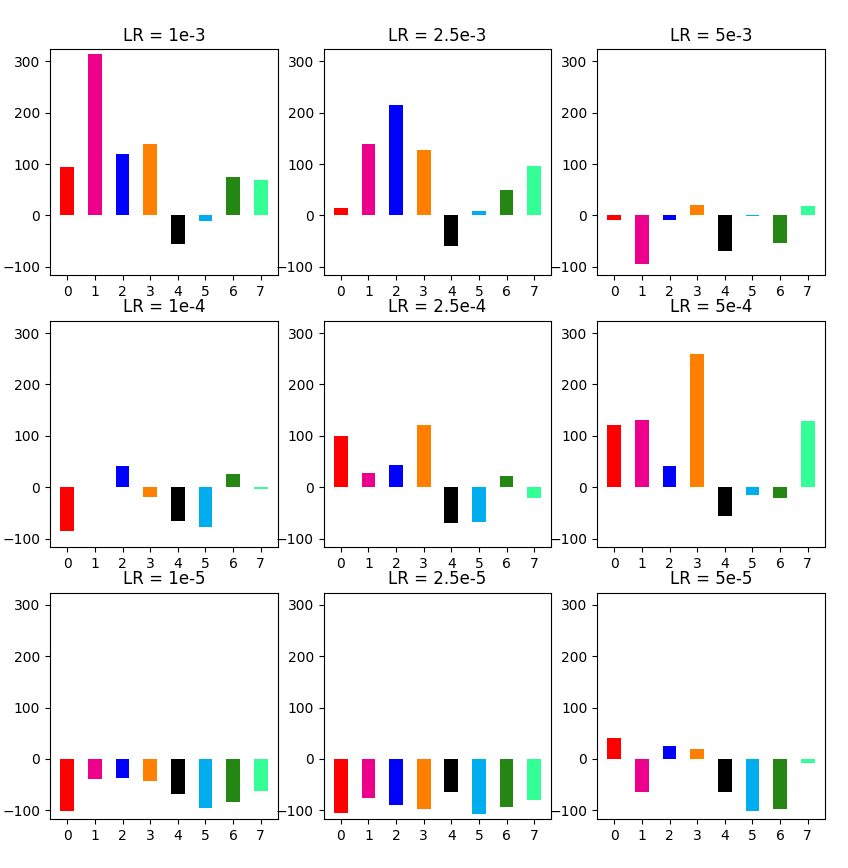
\includegraphics[width=0.8\textwidth]{images/chapter_4/DQN_search}
	\caption{Búsqueda exhaustiva de parámetros del algoritmo DQN ejecutando nueve procesos}
	\label{fig:dqn_search}
\end{figure}
